\chapter{Schramm-Loewner Evolutions}
\label{ch:sle}

The most exciting advances in natural sciences happen when two previously
unrelated or loosely related fields are brought together to give new insight
into old problems. That's what happened when Descartes and Fermat joined
algebra (which had just recently reached Europe) and geometry to form analytic
geometry~\cite{Stillwell2010}, an indispensable part of the modern science and
engineering mathematical toolbox. Or when Einstein applied the abstract and
esoteric non-Euclidian geometry to the physical world with his theory of
gravity.

The area of critical phenomena is fortunate enough to see this happen twice.
The first was the introduction of conformal invariance and conformal field
theory, which were first developed in the 50's by field theorists as a means of
creating exactly solvable toy models~\cite{Thirring1958}, but in the 80's were
very successfully used to compute the critical properties of several
two-dimensional systems~\cite{Nahm2000}. Conformal field theory, however, was
not free of criticism, specially from mathematicians. Notions like
renormalization and field operators are not well defined and often behave, as
Cardy puts it, ``according to rules that seem to be a matter of cultural
convention rather than rigorous logic''~\cite{Cardy2005}. That and the
inability of answering some very important questions~\cite{Langlands1994} led
mathematicians to search for other theories.

In 2000, a remarkable development happened when Oded Schramm published his
theory of Stochastic Loewner Evolutions~\cite{Schramm2000} (SLE). Combining
ideas from complex analysis and measure theory, SLE looks not at the fields
themselves, but at the random curves that the form the boundary of clusters.
This theory was an astounding success, not only rigorously reproducing
previously established results, but also answering long standing unsolved
problems, like Mandelbrot's conjecture that the boundary of a 2D Brownian
motion has fractal dimension of $4/3$~\cite{Lawler2001}.


\section{Loewner Equation}
\label{sec:le}

The ``Loewner Evolution'' part of SLE came much earlier, it was proposed in
1923 by Charles Loewner in the context of the Bieberbach
conjecture~\cite{Loewner1923}, which concerned some properties of Taylor
expansions of analytical function, and completely proved by de Branges in
1985~\cite{DeBranges1985}. The starting point of the process described by
Loewner is the Riemann mapping theorem~\cite{Ahlfors1979}. This theorem
guarantees the existence of a conformal transformation (as defined in
Section~\ref{ch:conf}) that maps any two regions of the complex plane into one
another, as long as these regions are simply connected, that is, they should
have no holes in them. The theorem also assures that the boundary of one region
gets mapped onto the boundary of the other. In other words, we can transform a
region of the complex plane into any shape we want by using a suitable
conformal map, as illustrated in Figure~\ref{fig:scmap}. Luckily conformal maps
are also bijective, so the inverse process is always possible too. In the
majority of cases there is no simple form for the map, but they can be
constructed at least numerically using Schwartz-Christoffel
maps~\cite{Driscoll2002}. There is no restriction for the form of the domains
involved, they can be as simple or complicated as desired, as long as they do
not have any holes in it, and their boundary has more than one point.

To define the Loewner process, we firstly take any simply connected domain $D$
which will serve as a standard domain. Now we imagine making a crack in this
domain, like shown in Figure~\ref{fig:diskfix}. This crack has no width, so it
can be described as a curve $\gamma$ which starts at some point $r_1$ at the
boundary $\partial D$ and ends at a point $r_2$ which may be an interior or
boundary point. As long as $\gamma$ does not touch itself, the cracked domain
$D\setminus\gamma$\footnote{$\cdot\setminus\cdot$ being the set-minus
    operator.} is also simply connected. Because of that, the Riemann mapping
theorem assure us that we can ``fix'' this crack by finding the conformal
transformation $g$ that maps the cracked domain into the uncracked standard
domain, or in math lingo $g:D\setminus\gamma\rightarrow D$. This is called a
\textit{uniformizing map}, and the crack  $\gamma$ goes by the more formal name
\textit{trace}. We distinguish two types of traces. If $r_2$ is an interior
point of $D$, the trace is said to be \textit{radial}, and if it belongs to the
boundary $\partial D$ it is called \textit{chordal}.

Let's parametrize the trace using a positive real parameter $t$ such that
$\gamma_{0}=r_1$ and $\gamma_{\infty}=r_2$. For now we'll leave the
parametrization choice free. We denote $\gamma_{[0,t]}$ the whole extent of the
trace from $\gamma_0$ up to the tip $\gamma_t$. Therefore, for every value of
$t$ we have a different uniformizing map
$g_t:D\setminus\gamma_{[0,t]}\rightarrow D$. We can imagine $t$ as a sort of
time, and the evolution of the tip $\gamma_t$ as a growth process.
An immediate question one might ask is, what is the relation between $D$,
$\gamma$ and the $g_t$? Are they uniquely defined? Is there a kind of equation
that relates these objects? Loewner's answer is ``yes'', as long as you're
willing to make a few compromises.

We can construct an equation for $g_t$ by shifting our attention from the trace
itself. You see, since the tip of the trace $\gamma_t$ is part of the boundary
of $D\setminus\gamma_{[0,t]}$, it will necessarily get mapped to a point
$U_t=g_t(\gamma_t)$ in the border of the standard domain $D$. If we follow the
time evolution of this point, we get a function
$U_t:\mathbb{R}^+\rightarrow\partial D$. This is called the \textit{driving
    function} of the trace in question. An schematic representation of the
whole process in shown Figure~\ref{fig:loewexplain}. In his work, Loewner
showed that the trace, the uniformizing on map, and the driving function are
connected by a differential equation.

Before we can write down this equation we need to make a series of assumptions.
One of them is to decide if we want to deal with radial or chordal traces.
Other is to determine the standard domain in which the trace will grow. In his
original work, Loewner chose the unit disc $\mathbb{D}=\{z||z|\leq1\}$, with
$\gamma_0=1$ and $\gamma_\infty=0$ for the radial case. For the chordal case,
the most commonly used domain is the upper half plane
$\HH=\{z|\mbox{Im}\{z\}\geq0\}$ with $\gamma_0=0$ and $\gamma_\infty=\infty$,
which offers the practicality that $\partial\HH=\mathbb{R}$, so the driving
function is real valued. In physical applications, it is much more common to
use the chordal version, and it's the version we'll focus here.
Figure~\ref{fig:radchord} show two examples of radial and chordal traces in
these domains.

In order to determine the chordal Loewner equation we need first to impose some
conditions on the conformal map $g_t$, otherwise there are an infinity of maps
that connect $\HH\setminus\gamma_{[0,t]}$ to $\HH$. To induce uniqueness, we
impose what is called a \textit{hydrodynamic normalization}. This means that
far from the origin, the uniformizing maps behave as
\begin{equation}
    \label{eq:hydro}
    g_{t}\left(z\right)\approx
    z+\frac{a\left(t\right)}{z}+O\left(z^{-2}\right)
    ,\,\,\,\,\,\,\,\,\,\,\,
    z\rightarrow\infty.
\end{equation}
This way, points at infinity get mapped into themselves. The coefficient $a(t)$
is called the half plane capacity, and can take any form as long as it obeys a
number of properties, including positivity, monotonicity and
continuity~\cite{Kager2004}. The choice of capacity is intrinsically connected
with the parametrization of the trace (the SLE time $t$) and it is far from a
trivial point, which has drawn some attention from
mathematicians~\cite{Lawler2011}. Here, we'll go with the most common choice of
$a(t)=2t$.

With all these properties laid out, the chordal Loewner equation takes the
(deceptively) simple form 
\begin{equation}
    \label{eq:loew}
    \partial_t g_t(z) = \frac{2}{g_t(z) - U_t}
    ,\,\,\,\,\,\,\,\,\,\,
    g_0(z)=z,
\end{equation}
where $U_t\in\mathbb{R}$ and the trace can be obtained by taking the limit
\begin{equation}
    \gamma_t = \lim_{z\rightarrow 0}g_t^{-1}\left(U_t + z\right),
\end{equation}
since the Loewner equation is not well defined for $g_t(z)=U_t$. The derivation
of Loewner's equation is outlined in Appendix~\ref{ch:proof} and a example of a
chordal trace obtained from it in Figure~\ref{fig:leexample}. Furthermore,
working only on the upper half plane seems restrictive, but remember that any
two domains can be mapped into one another through conformal transformations.
So to get the trace in a domain $D$ that connects two points $r_1, r_2 \in
\partial D$, all you have to do is to find the function $f:\HH\rightarrow D$,
where $f(0)=r_1$ and $f(\infty)=r_2$. Under similar assumptions, the radial
Loewner equation in the unit disc is
\begin{equation}
    \partial_{t}g_{t}\left(z\right)=
    g_{t}\left(z\right)
    \frac{e^{iU_{t}}+g_{t}\left(z\right)}
         {e^{iU_{t}}-g_{t}\left(z\right)}
    ,\,\,\,\,\,\,\,\,\,\,
    g_0(z)=z.
\end{equation}
with $U_t\in\mathbb{R}$. Figure~\ref{fig:radchord} shows the trace
obtained in both cases for a simple driving function.

Not surprisingly, the topological and geometric properties of the trace
$\gamma_t$ are intimately connected with the analytical properties of the
driving function $U_t$. Some properties include~\cite{Gruzberg2004}:
\begin{enumerate}
    \item if $U_t$ is smooth, with a derivative well defined, then $\gamma_t$
        never intersects itself;
    \item if $U_t$ is periodic, $\gamma_t$ is self-similar;
    \item if $U_t$ is H\"older continuous with exponent $1/2$ with constant
        larger than 4, meaning that there is a finite constant $C$ such that
        \begin{equation}
            \label{eq:holder}
            4<\lim_{s\rightarrow0^{+}}\left|
                \frac{U_{t-s}-U_{t}}{s^{1/2}}\right|
            <C,
        \end{equation}
        then the trace does touch itself.
\end{enumerate}
This last one might require some clarification. We established that the Riemann
mapping theorem is valid only for simply connected domains. If the trace touches
itself at an instant $\tau$, then $D\setminus\gamma_{[0,t\geq\tau]}$ is not
simply connected, and the existence of $g_t$ cannot be guaranteed. This
confusion comes from an innocent omission made at the beginning of this
section (made to keep things simple). The uniformizing map that satisfy the
Loewner equation does not in fact map $D\setminus\gamma_{[0,t]}$ to $D$. It
actually maps $D\setminus K_t$ to $D$, where the \textit{hull} $K_t$ is the set
comprising the trace $\gamma_{[0,t]}$ \textit{and} all the space trapped inside
the loops formed when the trace touches itself. One can easily see that $K_t$
is always simply connected and if the trace is simple $K_t = \gamma_{[0,t]}$.

The overall behavior of the trace follows that of the driving function, so a
very complicated $U_t$ tend to generate very intricate traces. One could
imagine a driving function that has a discontinuous jump, for example. In this
case, the trace will have also display a break, starting a new branch coming
out of the real line or from the old segment depending on the size of the
discontinuity, giving the trace a tree-like aspect, like shown in
Figure~\ref{fig:discle}.


\begin{figure}
\begin{center}
    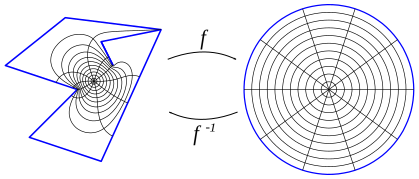
\includegraphics[scale=1.0]{chapters/ch4-sle/figs/scmap}
\end{center}
\caption{The Riemann mapping theorem guarantees the existence of at least one
    conformal mapping $f$ that maps any two simply connected two-dimensional
    domains. In $2D$ any conformal map is invertible. Generated using th
    Schwarz-Christoffel toolbox for MATLAB~\cite{Driscoll2005}.}
\label{fig:scmap}
\end{figure}


\begin{figure}
\begin{center}
    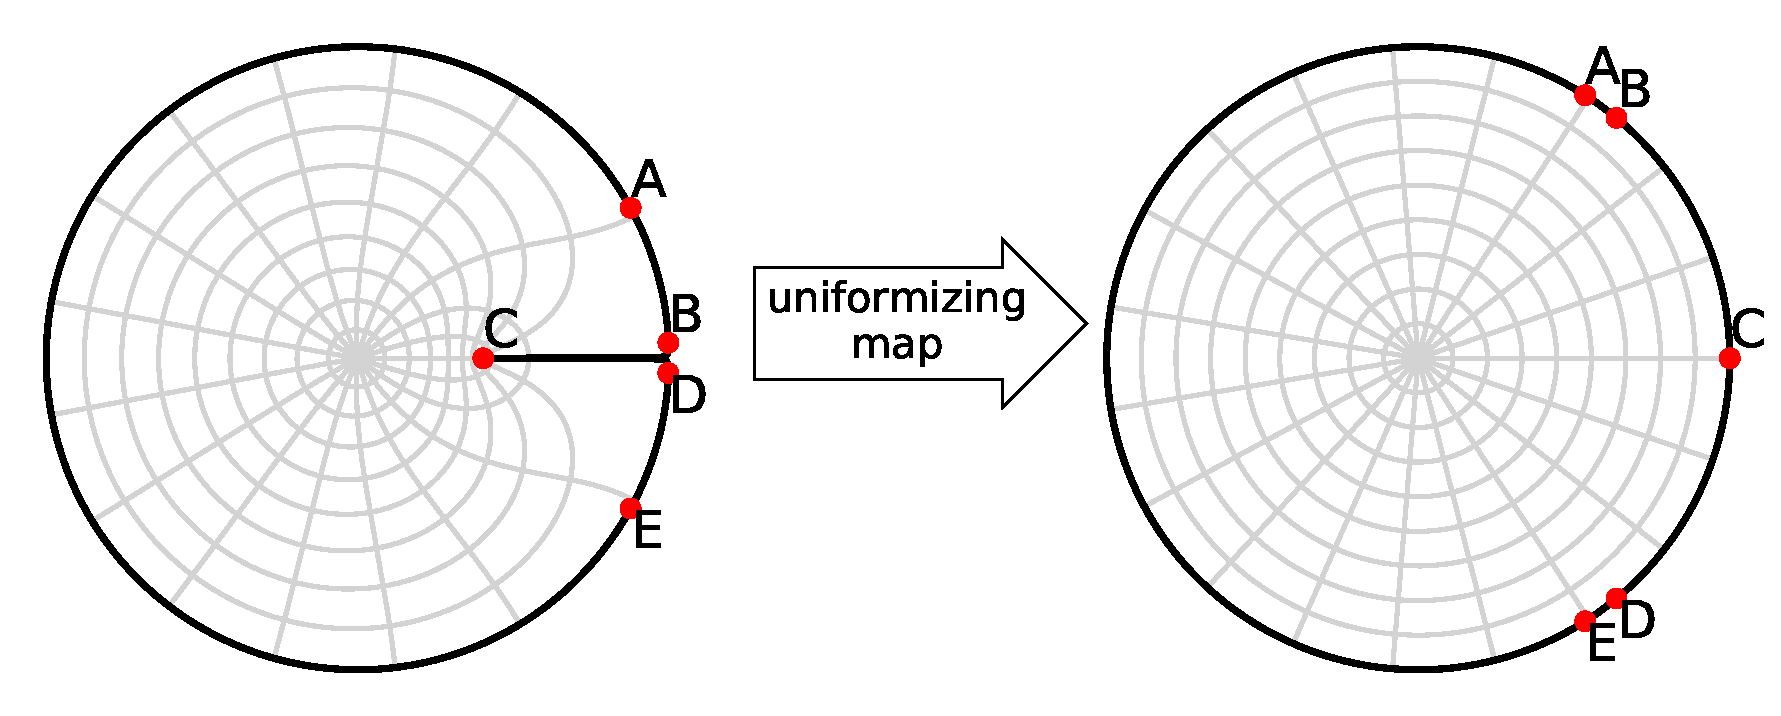
\includegraphics[width=\textwidth]{chapters/ch4-sle/figs/diskfix}
\end{center}
\caption{Using a suitable conformal transformation it is possible to remove
    a slit in the domain, mapping it to the circular boundary. Points close
    to each other in the slitted domain (B and D) get mapped far apart in
    the one without the slit.}
\label{fig:diskfix}
\end{figure}

\begin{figure}
\begin{center}
    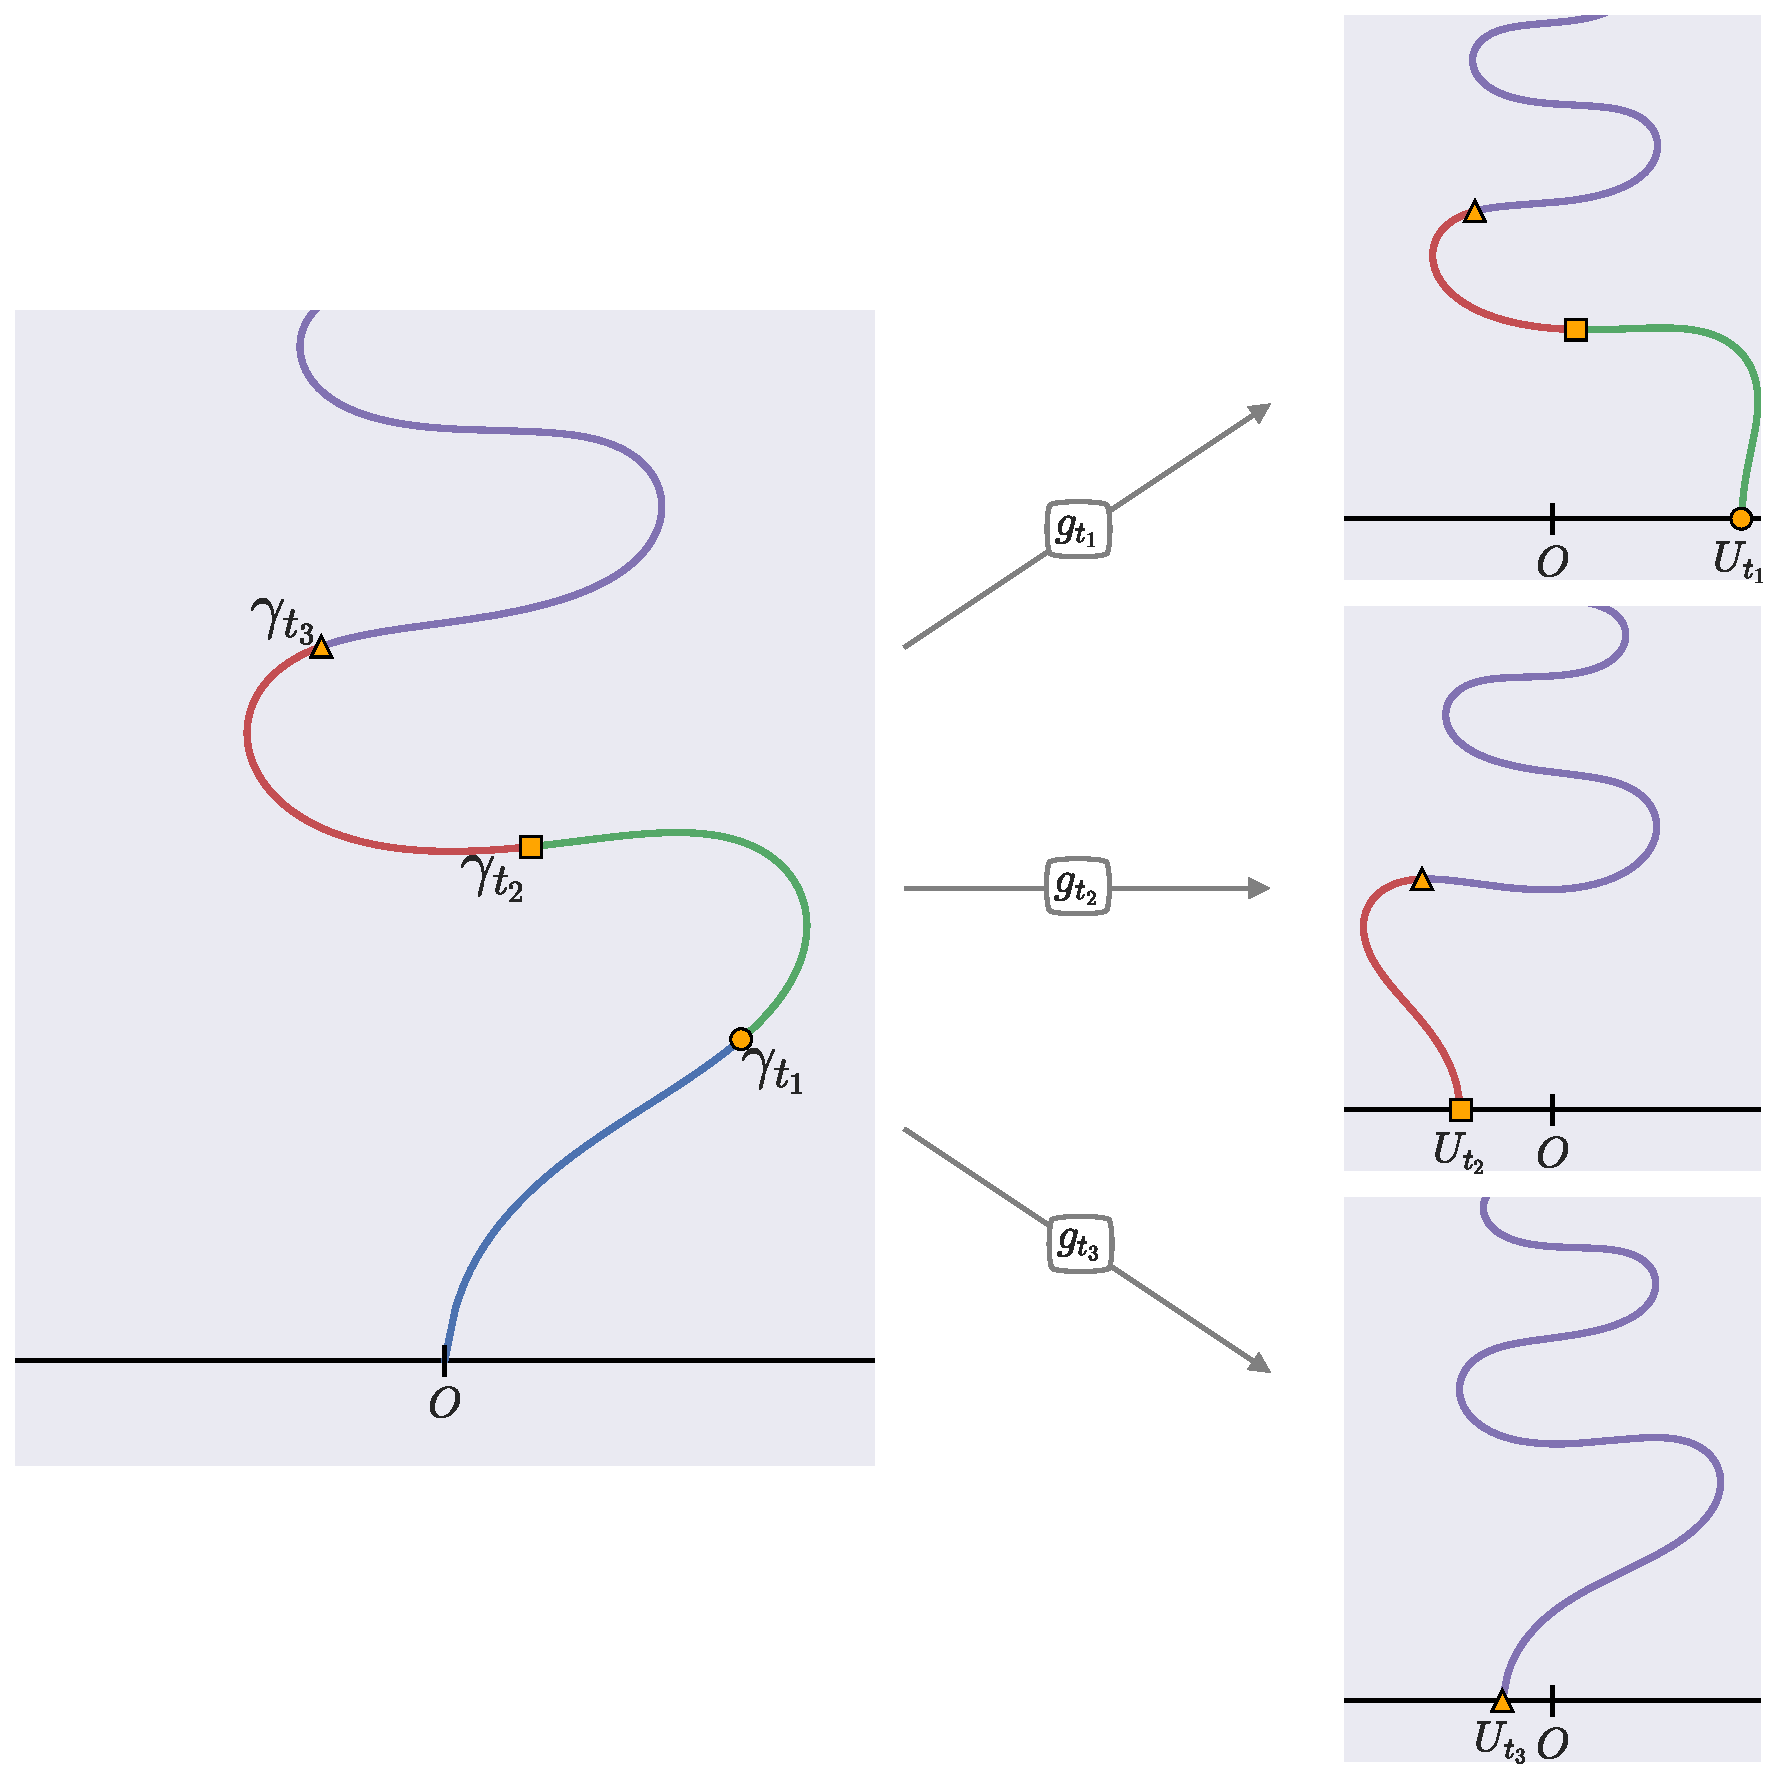
\includegraphics[scale=0.4]{chapters/ch4-sle/figs/loewexplain}
\end{center}
\caption{How the chordal Loewner evolution works. We define the trace $\gamma$
    parametrized by a time $t$. At each time instant there is a conformal map
    $g_t$ that maps the upper half plane minus the trace up to time $t$ to the
    upper half plane itself, that is, $g_t:\HH\setminus\gamma_{[0,t]}
    \rightarrow\HH$. The tip of the trace always get mapped to the real line.
    If we track the point where the tip is mapped, we get a function $U_t$
    called driving function, that is $U_t=g_t\left(\gamma_t\right)$.
    The trace, driving function and uniformizing maps are all related through
    Loewner's equation (Eq.~\ref{eq:loew}).}
\label{fig:loewexplain}
\end{figure}

\begin{figure}
\begin{center}
    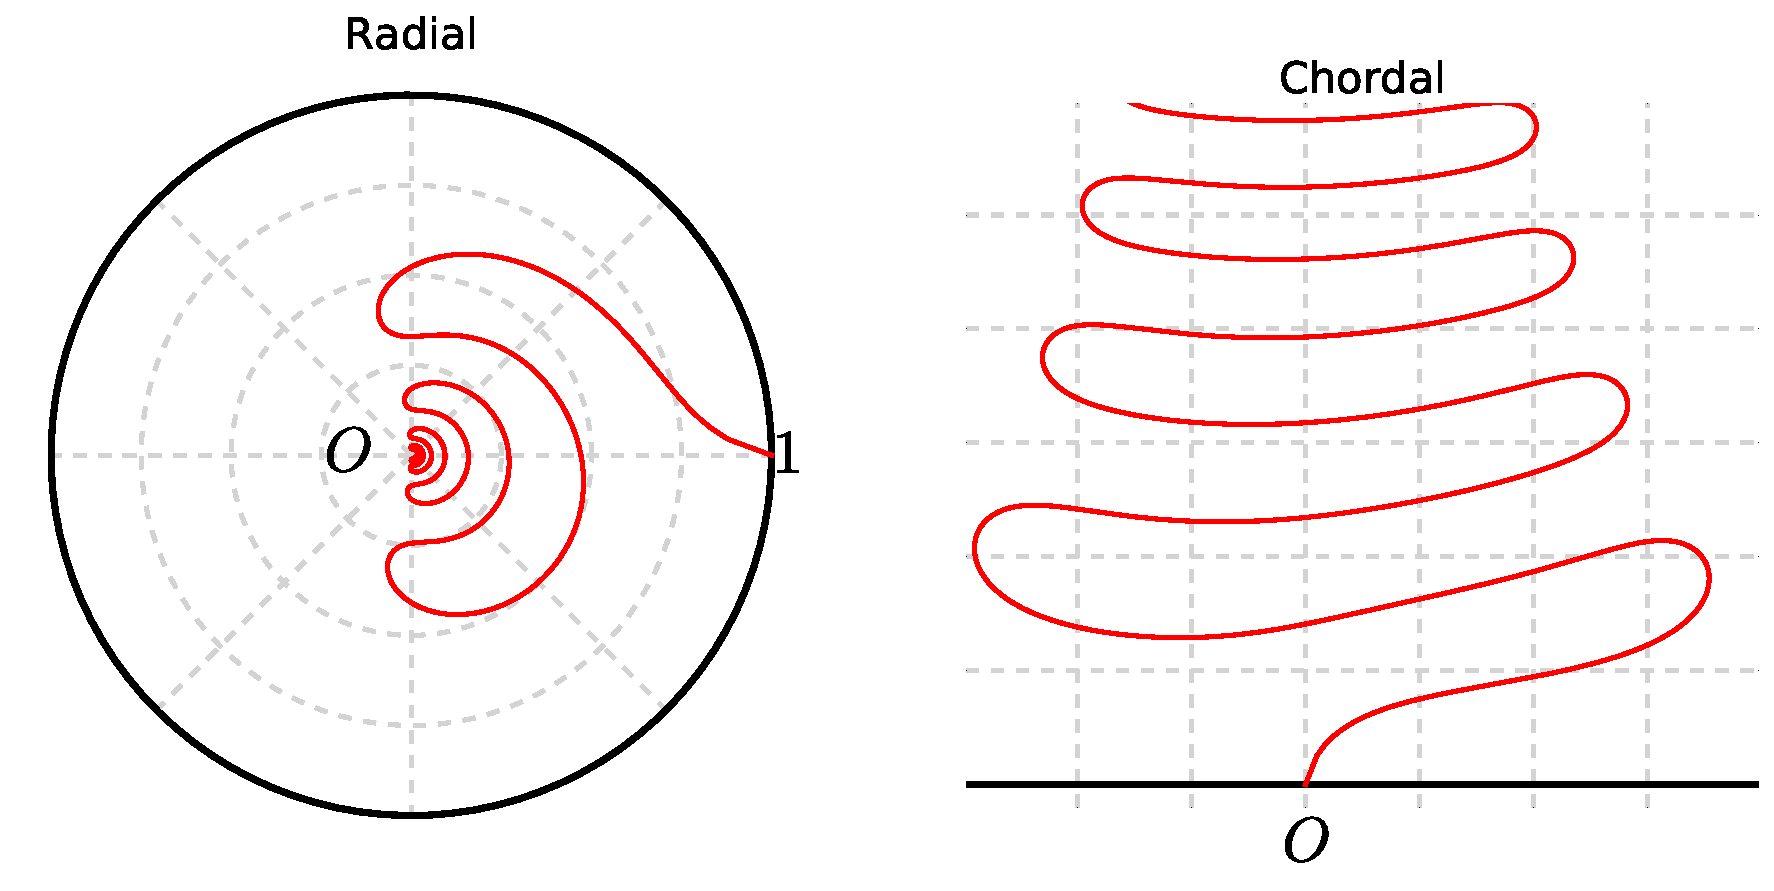
\includegraphics[scale=0.4]{chapters/ch4-sle/figs/radchord}
\end{center}
\caption{Radial versus chordal Loewner traces generated using the same driving
    function $U_t=2\sin(2\pi t)$ (in the radial case you have to use
    $\exp(iU_t)$). Radial curves are contained inside the unit circle
    $\mathbb{D}=\{z||z|\leq1\}$ and start at $z=1$ growing towards the origin.
    Chordal traces are contained in the upper half plane
    $\HH=\{z|\mbox{Im}\{z\}\geq0\}$ starting at the origin and growing towards
    infinity.}
\label{fig:radchord}
\end{figure}

\begin{figure}
\begin{center}
    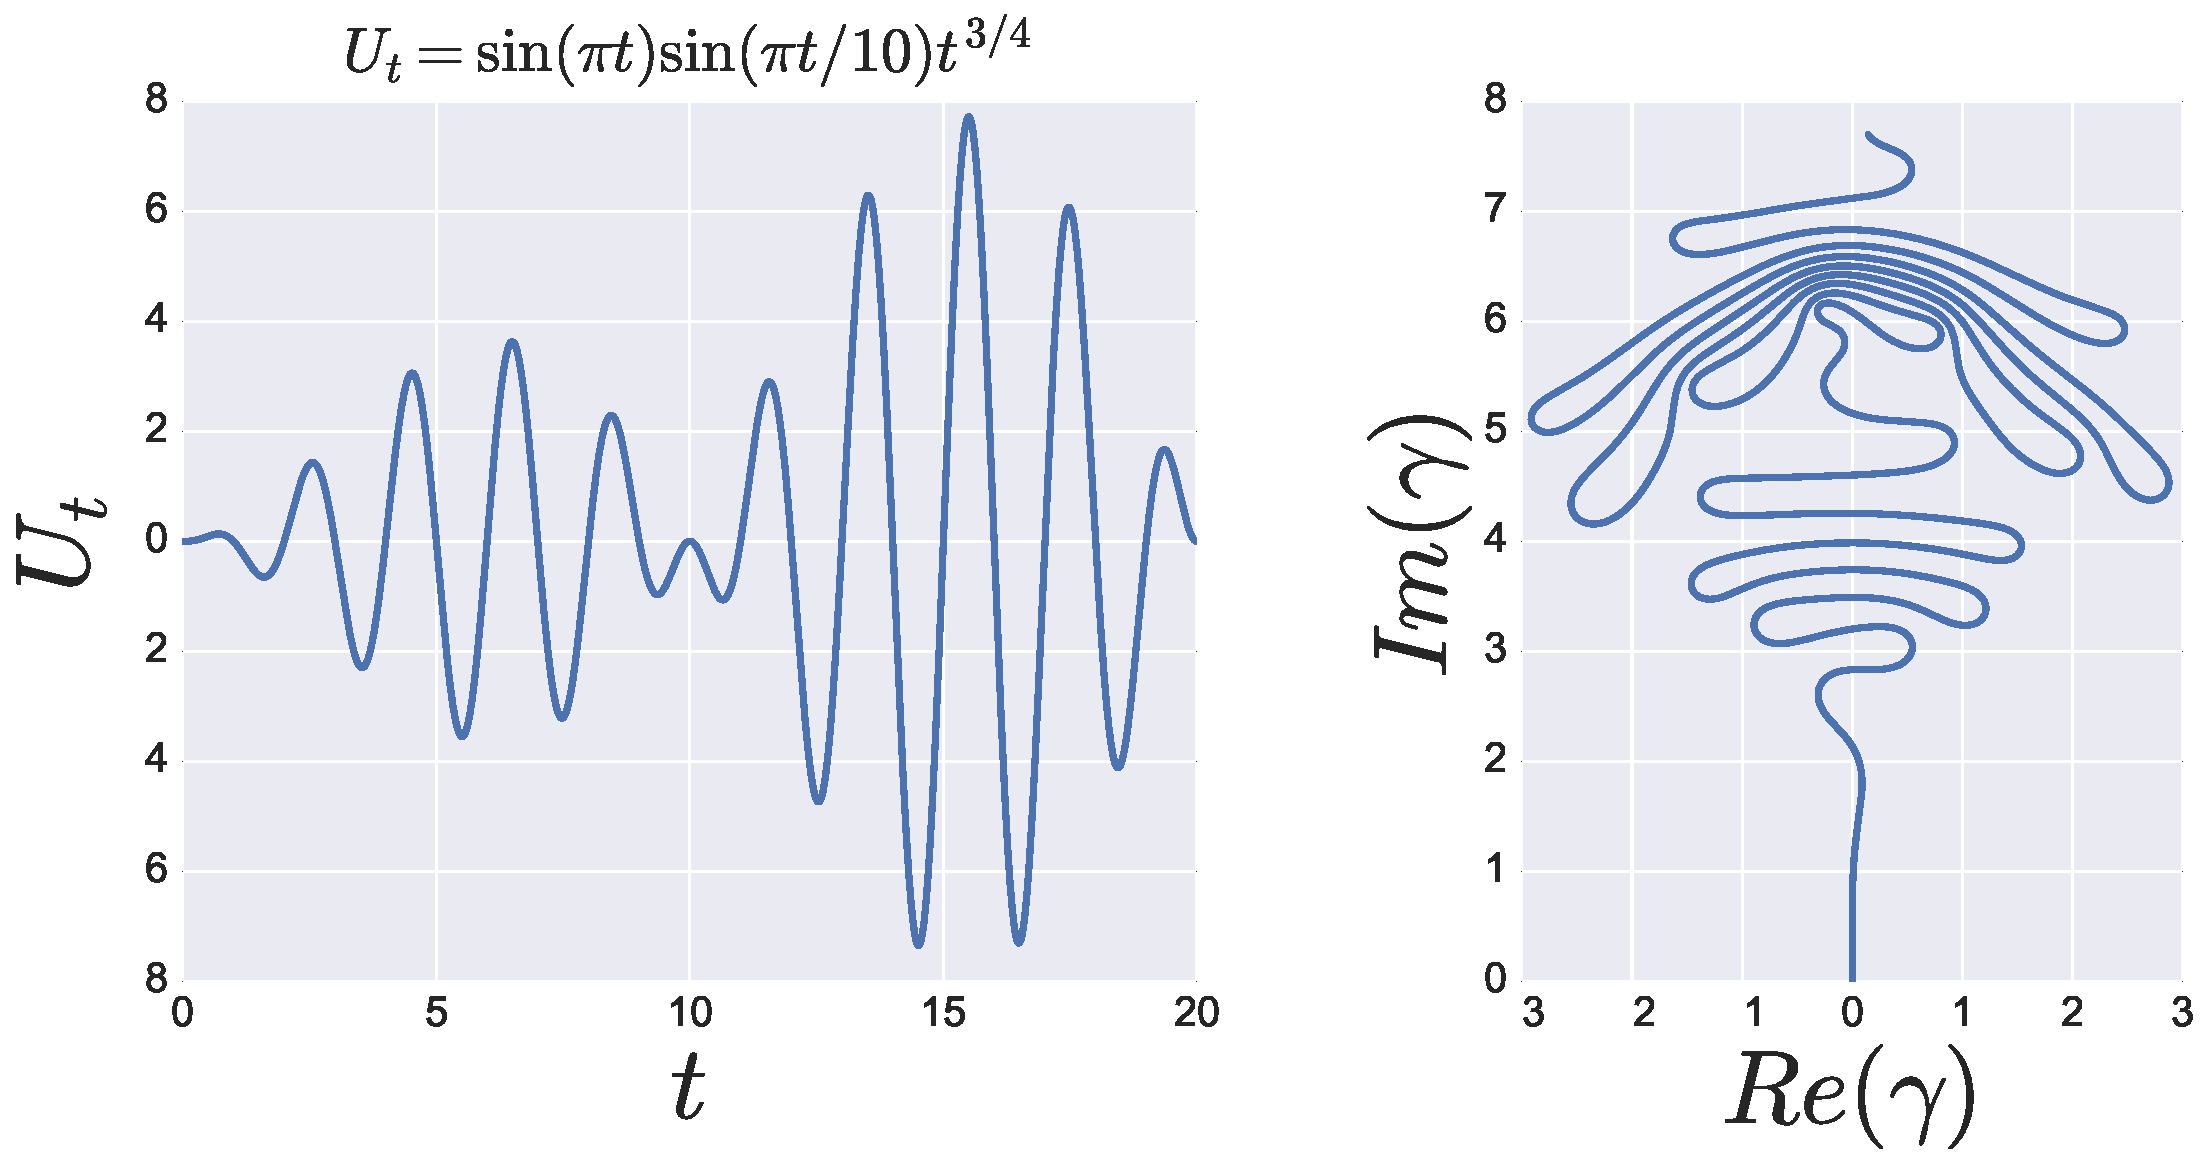
\includegraphics[width=\textwidth]{chapters/ch4-sle/figs/leexample}
\end{center}
\caption{Example of a Loewner trace generated by the driving function
    $U_t=\sin(\pi t)\sin(\frac{\pi t}{10})t^{3/4}$. The trace $\gamma$ is
    defined by the relation $\gamma_t = g_t^{-1}(U_t)$, where $g_t$ is the
    solution of the Loewner differential equation (Eq.~\ref{eq:loew}).}
\label{fig:leexample}
\end{figure}

\begin{figure}
\begin{center}
    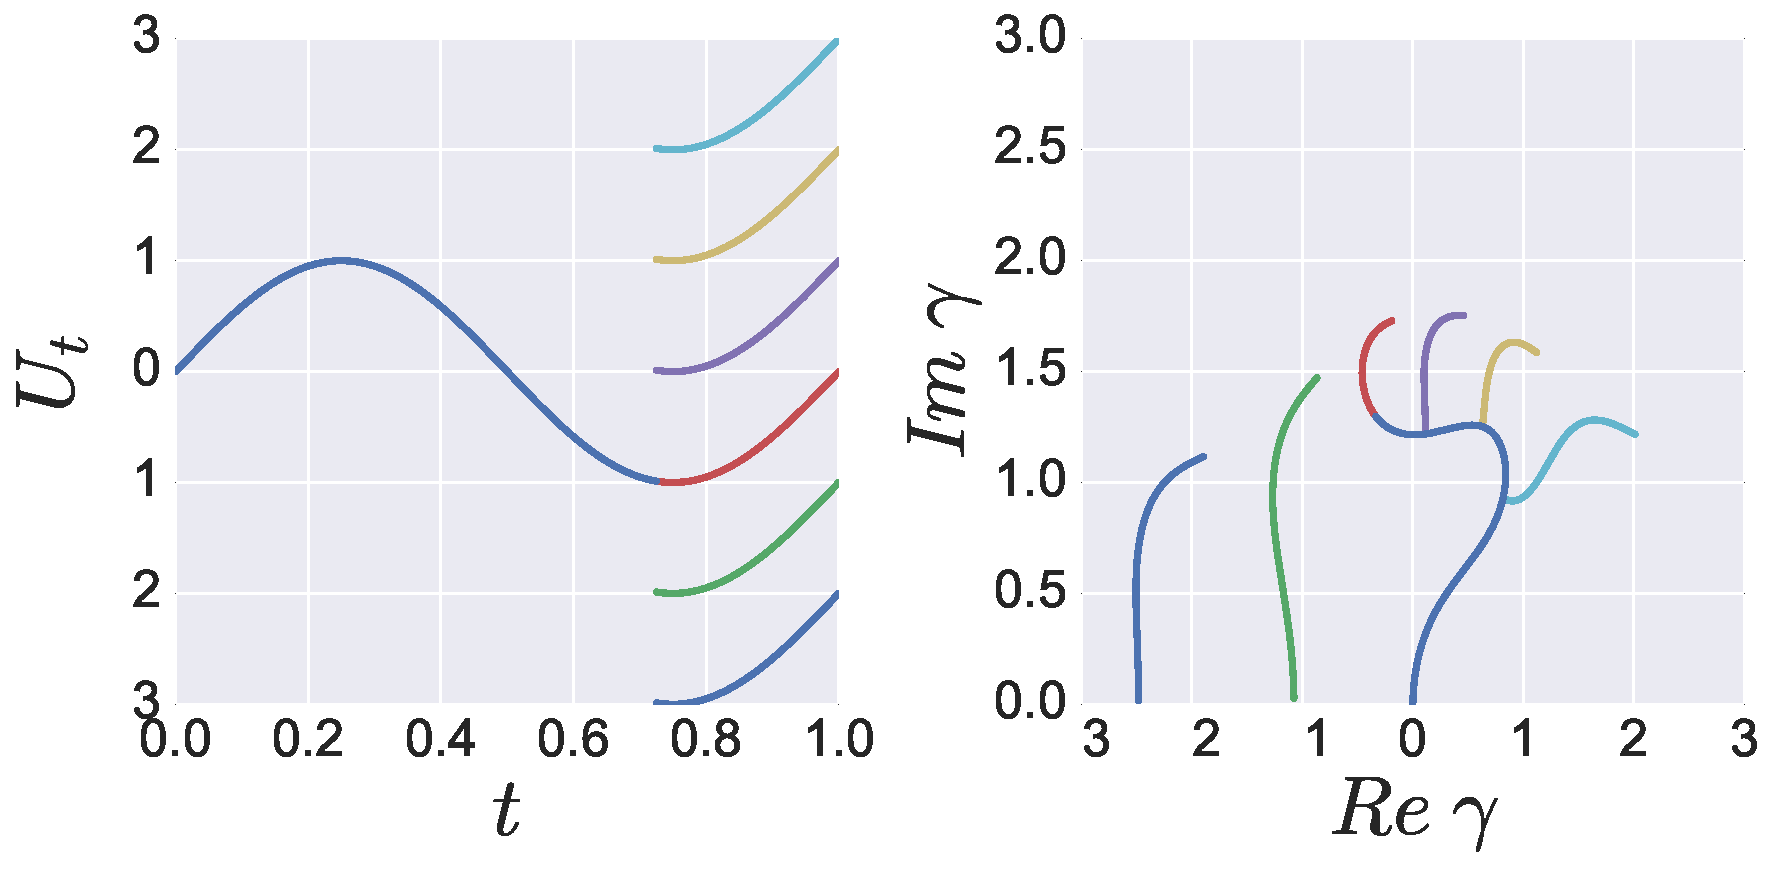
\includegraphics[width=\textwidth]{chapters/ch4-sle/figs/discle}
\end{center}
\caption{The Loewner trace driven by discontinuous functions with several sizes
    of discontinuity. The resulting trace is also discontinuous taking a
    tree-like structure, where new branches can start at real line or at the
    older branches depending on the size of the discontinuity.}
\label{fig:discle}
\end{figure}


\section{Stochastic Loewner Evolutions}
\label{sec:sle}

A big breakthrough in the area of critical phenomena happened when Oded Schramm
used Loewner evolutions to study the interfaces that form in critical systems,
like the perimeter of a percolation cluster. He did that by showing that all
properties of conformally invariant models are codified in a family of Loewner
evolutions driven by a fairly simple driving function. In this section we'll
give an outline of this theory, but there's an abundance of material for the
reader interested in digging deeper~\cite{Cardy2005, Kager2004, Henkel2012}.

If we want to describe conformally invariant critical systems using
Loewner processes, we need to redefine the concept conformal invariance. The
definition given in terms of the covariance of field operators
(Eq.~\ref{eq:cinv}) does not translate well into the framework of Loewner
evolutions because there's no way to incorporate the notion of field. Instead
we need to define it in terms of the curves that form the boundaries of
clusters, which are meant to be the traces. To do that we take a measure theory
approach (the more general mathematical theory of probability)~\cite{Ash2000}.
In this context, we define conformal invariance as follows: let $f$ be a
conformal map between two domains $D$ and $D'$ such that $D'=f(D)$, then the
measure over the set of traces that connect two points $z,w\in\partial D$
should behave like~\cite{Cardy2005}
\begin{equation}
    \newcommand{\pp}[1]{\left(#1\right)}
    f\circ\mu_D\pp{z,w} = \mu_{f(D)}\pp{f\pp{z}, f\pp{w}}.
\end{equation}
That is to say, suppose you want to generate a curve in a, say, triangular
region. You can do this in two ways, one by simply applying you lattice model
to the triangular domain, or you can apply the lattice model in a square domain
and then conformally map the resulting trace to a triangular domain. Conformal
invariance states that, in the \textit{continuum limit}, these two processes
are statistically identical, as illustrated in Figure~\ref{fig:confinv}. Here
we used the term \textit{measure} instead of probability distribution, because
the latter cannot be actually be defined for traces in the continuum limit, but
the more general concept of measure can be applied.

Conformal invariance, however, is not enough to pinpoint a general driving
function for critical systems. In his work, Schramm identified another
fundamental property that lattice models must have in the continuum limit, and
indeed tend to obey. It is called \textit{domain Markov property}, and refers
to the measure of a trace segment $\gamma_2$ conditioned by a
fixed initial segment $\gamma_1$,
\begin{equation}
    \newcommand{\pp}[1]{\left(#1\right)}
    \mu_D\pp{\gamma_2|\gamma_1} = \mu_{D\setminus\gamma_1}\pp{\gamma_2}.
\end{equation}
It means that the conditional measure of family of curves $\gamma_2$ that have the
same start $\gamma_1$ in a domain $D$ is the same as that of $\gamma_2$ in
the same domain with $\gamma_1$ removed, that is, $D\setminus\gamma_1$.
In the same line of conformal invariance, domain Markov property can be
understood in the following way: if you use a model to generate a set of curves
in $D$ that all have the same start $\gamma_1$, the curves $\gamma_2$ obtained
would have the exact same properties as if you generated the curves by applying
the model to $D\setminus\gamma_1$. And just like conformal invariance, this is
only expected to hold in the continuum limit. A visual explanation can be seen
in Figure~\ref{fig:dmp}.

The interfaces present in critical systems are usually random curves, so it is
only safe to assume that their driving functions should also be stochastic
processes. The climax is Schramm's work was the proof that systems that obey
conformal invariance and domain Markov property, as defined above, can only
have as a driving function
\begin{equation}
    U_{t}=\sqrt{\kappa}B_{t},
\end{equation}
where $B_t$ is a Brownian motion, also known as Wiener process.
It is defined as having the following properties~\cite{Durrett1996}:
\begin{itemize}
    \item $B_0=0$;
    \item The increments $B_t-B_s$ with any $t>s$ are always independent from
        one another;
    \item The increments $B_t-B_s$ with any $t>s$ are distributed according to
        a normal distribution with zero mean and variance $\sigma^2=t-s$;
    \item $B_t$ is almost surely continuous.
\end{itemize}
This is a striking result. Using only a family of driving functions with a
single parameter, we're able to describe all properties of many criticality
models. In the inaugural paper of SLE, Schramm showed that loop-erased random
walks (random walks with the loops removed in chronological order) and uniform
spanning trees converge to SLE with $\kappa=2$ and $\kappa=8$ respectively.
Figure~\ref{fig:sleexample} shows a realization of SLE with $\kappa=2$.

Mathematicians and physicists were quickly drawn to this new theory, unveiling
various interesting properties. One that stands out is how the trace looks with
different values of $\kappa$~\cite{Rohde2011}. You see, the Brownian motion is
basically a function that varies randomly with time. This random variation
gives the wiggly aspect of the trace, as seen in Figure~\ref{fig:sleexample}.
This means that the higher the value of $\kappa$, the larger will be the
variations of the Brownian motion, and the more wiggly the trace will be. When
the value of $\kappa$ is less or equal than $4$ the trace won't wiggle so
wildly to the point of touching itself. So in this case the trace is a simple
curve, as we already suggested in the last section with Eq.~\ref{eq:holder}.
When $\kappa>4$, however, the trace almost surely touch itself in all length
scales, to the point that the hull (the trace plus the regions inside the loops
it forms) eventually swallows the whole upper half plane. If $\kappa\geq8$ not
only the trace touches itself, but it does so on \textit{every} point of the
domain, so there is no point in $\HH$ that does not eventually belong to the
trace, we say the curve is space filling. The general aspect of the tree phases
can be seen in Figure~\ref{fig:kappa}.

The behavior of the trace in each of the three distinct phases is closely
related to its fractal dimension. The fractal dimension $d_f$ of a curve if
usually defined by counting the number $N$ of circles of radius $\epsilon$
needed to cover the whole curve. This should behave as~\cite{Mandelbrot1983}
\begin{equation}
    N\sim \epsilon^{-d_f}.
\end{equation}
The relationship between $\kappa$ and the fractal dimension was determined by
Beffara~\cite{Beffara2008} and given by
\begin{equation}
    d_f=\min\left(1+\frac{\kappa}{8},2\right).
\end{equation}
We see that for $\kappa\geq 8$ implies that $d_f=2$, which is exactly what we
would expect from a space filling curve. You can see several realizations of
SLE for different values of $\kappa$ and how the trace and its fractal
dimension behave in Figure~\ref{fig:slefracdim}.

Some other properties are useful to know if one is trying to determine if a
model can be represented by a SLE, specially if the investigation is numerical.
The probability that a point $z=|z|e^{i\theta}$ is to the left of the trace,
for instance, depends only on $\theta$ and is given by
\begin{equation}
    \label{eq:lpp}
    P=\frac{1}{2}+
    \frac{\Gamma\left(4/\kappa\right)}
         {\sqrt{\pi}
          \Gamma\left(\left(8-\kappa\right)/\left(2\kappa\right)\right)}
    \cot\left(\theta\right)
    {}_{2}F_{1}\left(\frac{1}{2},\frac{4}{\kappa},\frac{3}{2};
        -\cot^{2}\theta\right),
\end{equation}
where ${}_2F_1$ is the Gaussian hypergeometric function. A good evidence that a
model can be described by SLE is to generate various traces and estimate the
value of $\kappa$ using equation~\ref{eq:lpp}. This value should be consistent
with the coefficient of diffusion of the computed driving function (see
Section~\ref{sec:num} for how to compute the drive of a trace), which should
behave as
\begin{equation}
    \left\langle U_{t}^{2}\right\rangle =\kappa t.
\end{equation}

The point of contact between statistical physics and SLE happen at the
central charge of a conformal field theory. Bauer and Bernard~\cite{Bauer2002}
showed that $\kappa$ and $c$ are connected by the relation
\begin{equation}
    c=\frac{\left(3\kappa-8\right)\left(6-\kappa\right)}{2\kappa}.
\end{equation}
One might notice that each central charge value corresponds to two values of
$\kappa$, namely $\kappa$ and $16/\kappa$. This is connected the notion of
duality of SLE, first suggested by Duplantier~\cite{Duplantier2000} who noticed
that if we remove the loops of an SLE trace with $\kappa>4$ we would be left
with yet another SLE trace (at least locally) this time with
$\tilde{\kappa}=16/\kappa$. This was eventually proved for that case
$\kappa=6$~\cite{Beffara2004}, which has a dual $\tilde{\kappa}=8/3$, suspected
to be the same as the self-avoiding walk.

Since Schramm's first publication, various lattice models have been shown to
converge to SLE, which is a testament to the success of the theory. Some of the
values of $\kappa$ identified include
\begin{itemize}
    \item $\kappa=2$: loop-erased random walk~\cite{Schramm2000};
    \item $\kappa=8/3$: suspected to be self-avoiding walk~\cite{Kennedy2002},
        proved to be the border of a 2D random walk~\cite{Lawler2001};
    \item $\kappa=3$: cluster boundaries of the Ising model~\cite{Chelkak2014};
    \item $\kappa=4$: harmonic explorer~\cite{Schramm2005};
    \item $\kappa=6$: boundaries of percolation clusters~\cite{Smirnov2001b};
    \item $\kappa=8$: uniform spanning trees~\cite{Schramm2000}.
\end{itemize}
Furthermore, there's several models that have been conjectured to be
conformally invariant and have their own value of of $\kappa$ estimated
numerically. These include 2D and 3D turbulence~\cite{Bernard2006,
Thalabard2011}, shortest path of percolation clusters~\cite{Pose2014} and
watersheds~\cite{Daryaei2012}.

\begin{figure}
\begin{center}
    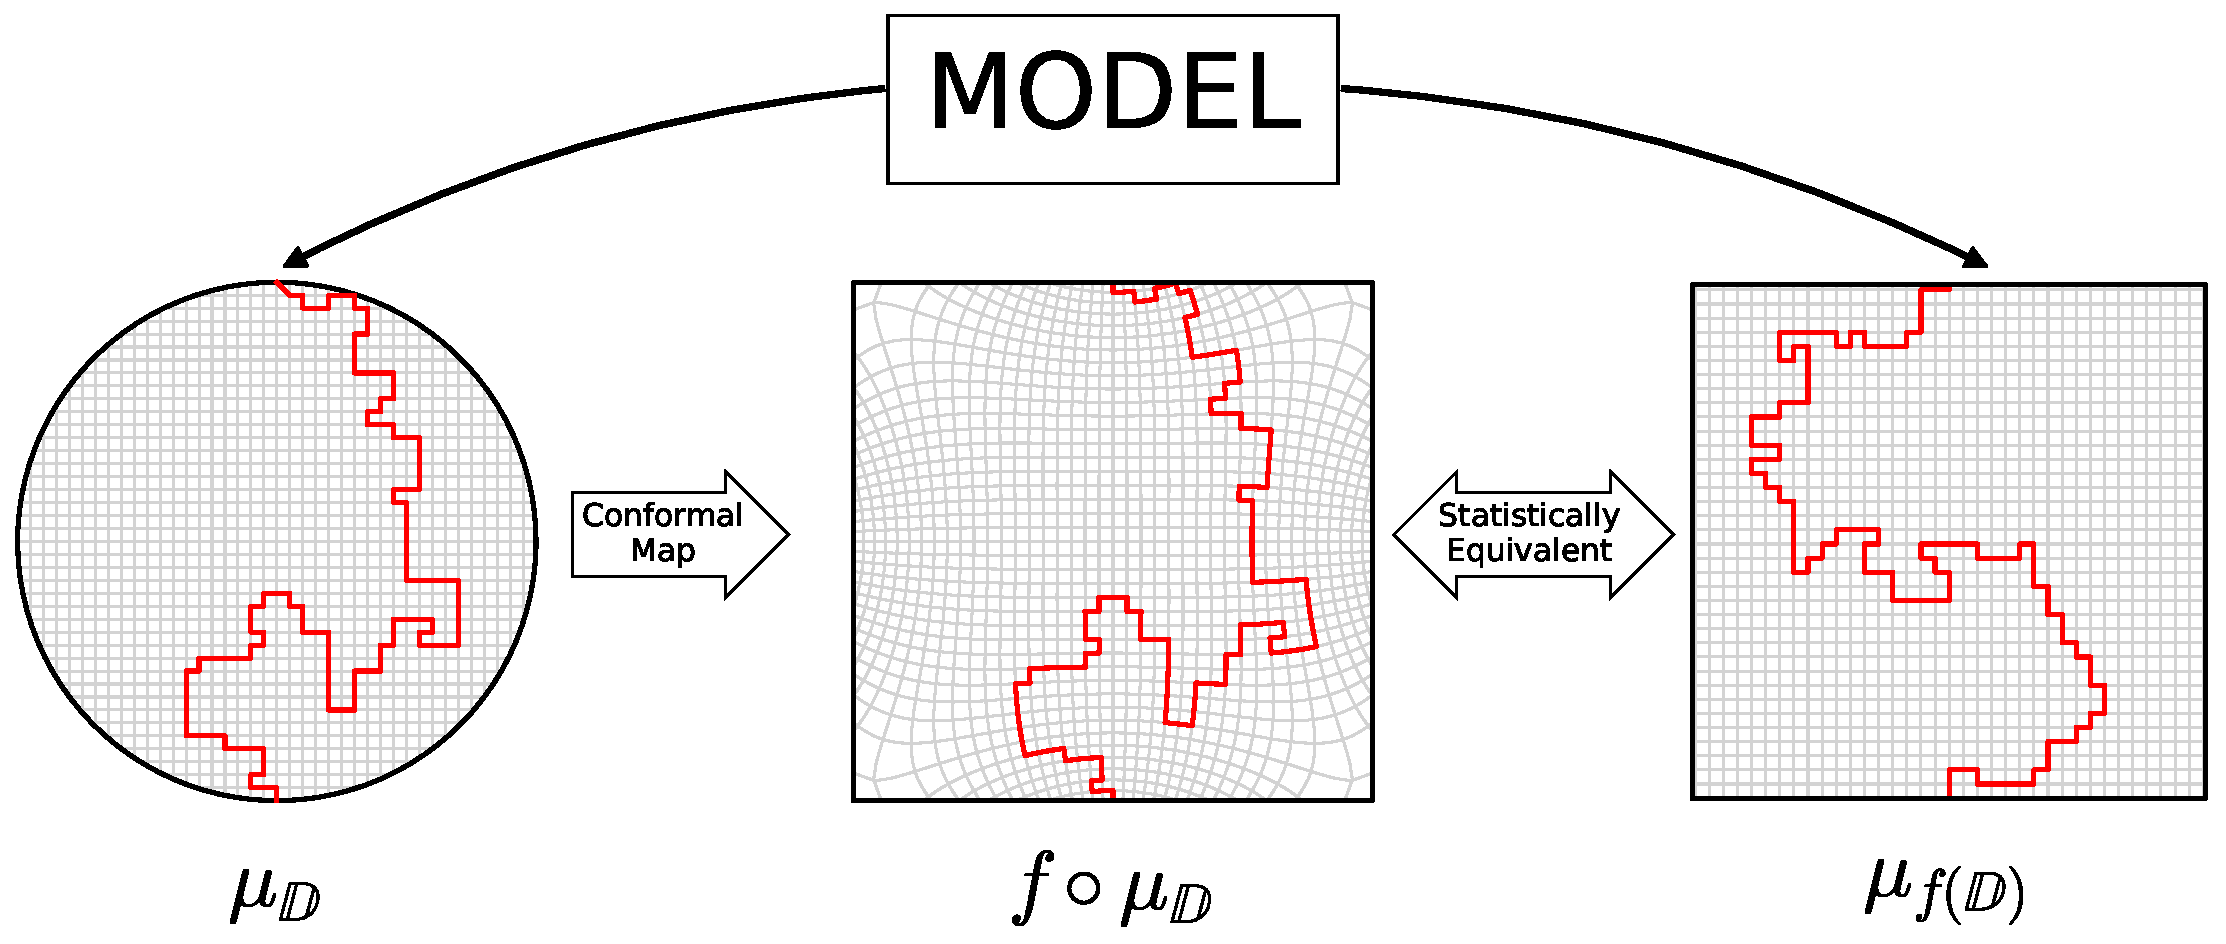
\includegraphics[width=\textwidth]{chapters/ch4-sle/figs/sle_confinv}
\end{center}
\caption{In the context of SLE, conformal invariance is defined in terms of the
    distribution of traces. For example, let $f$ be a conformal map from the
    unit disk $\mathbb{D}$ to a square domain $f(\mathbb{D})$, then the
    distribution $f\circ\mu_\mathbb{D}$ of the traces generated in $\mathbb{D}$
    and mapped to $f(\mathbb{D})$ should be the same as the distribution
    $\mu_{f(\mathbb{D})}$ of the traces generated directly in the square
    domain, in the continuum limit.}
\label{fig:confinv}
\end{figure}

\begin{figure}
\begin{center}
    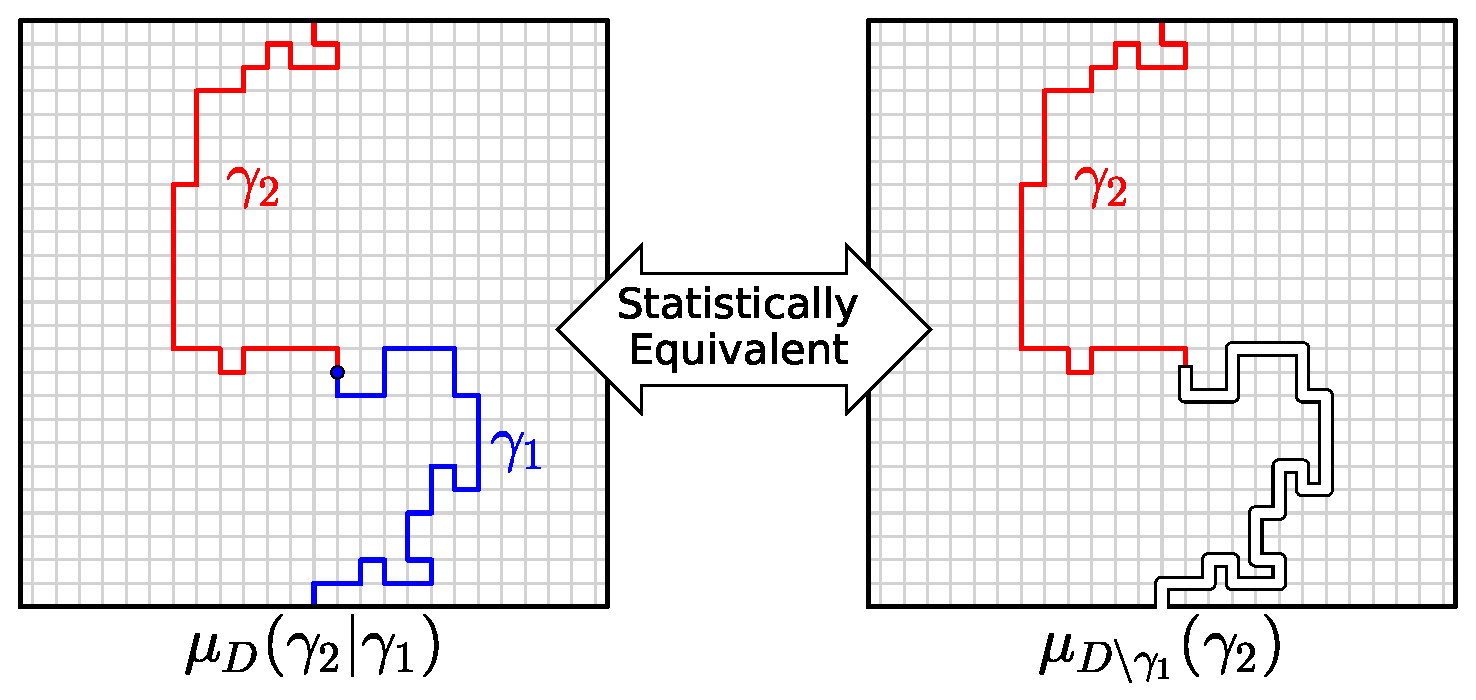
\includegraphics[width=\textwidth]{chapters/ch4-sle/figs/sle_dmp}
\end{center}
\caption{The domain Markov property states that the conditional distribution of
    $\gamma_2$ given a fixed $\gamma_1$ in a domain $D$,
    $\mu_D(\gamma_2|\gamma_1)$, is the same of $\gamma_2$ in the same domain
    with $\gamma_1$ removed, that is, $\mu_{D\setminus\gamma_1}(\gamma_2)$.}
\label{fig:dmp}
\end{figure}

\begin{figure}
\begin{center}
    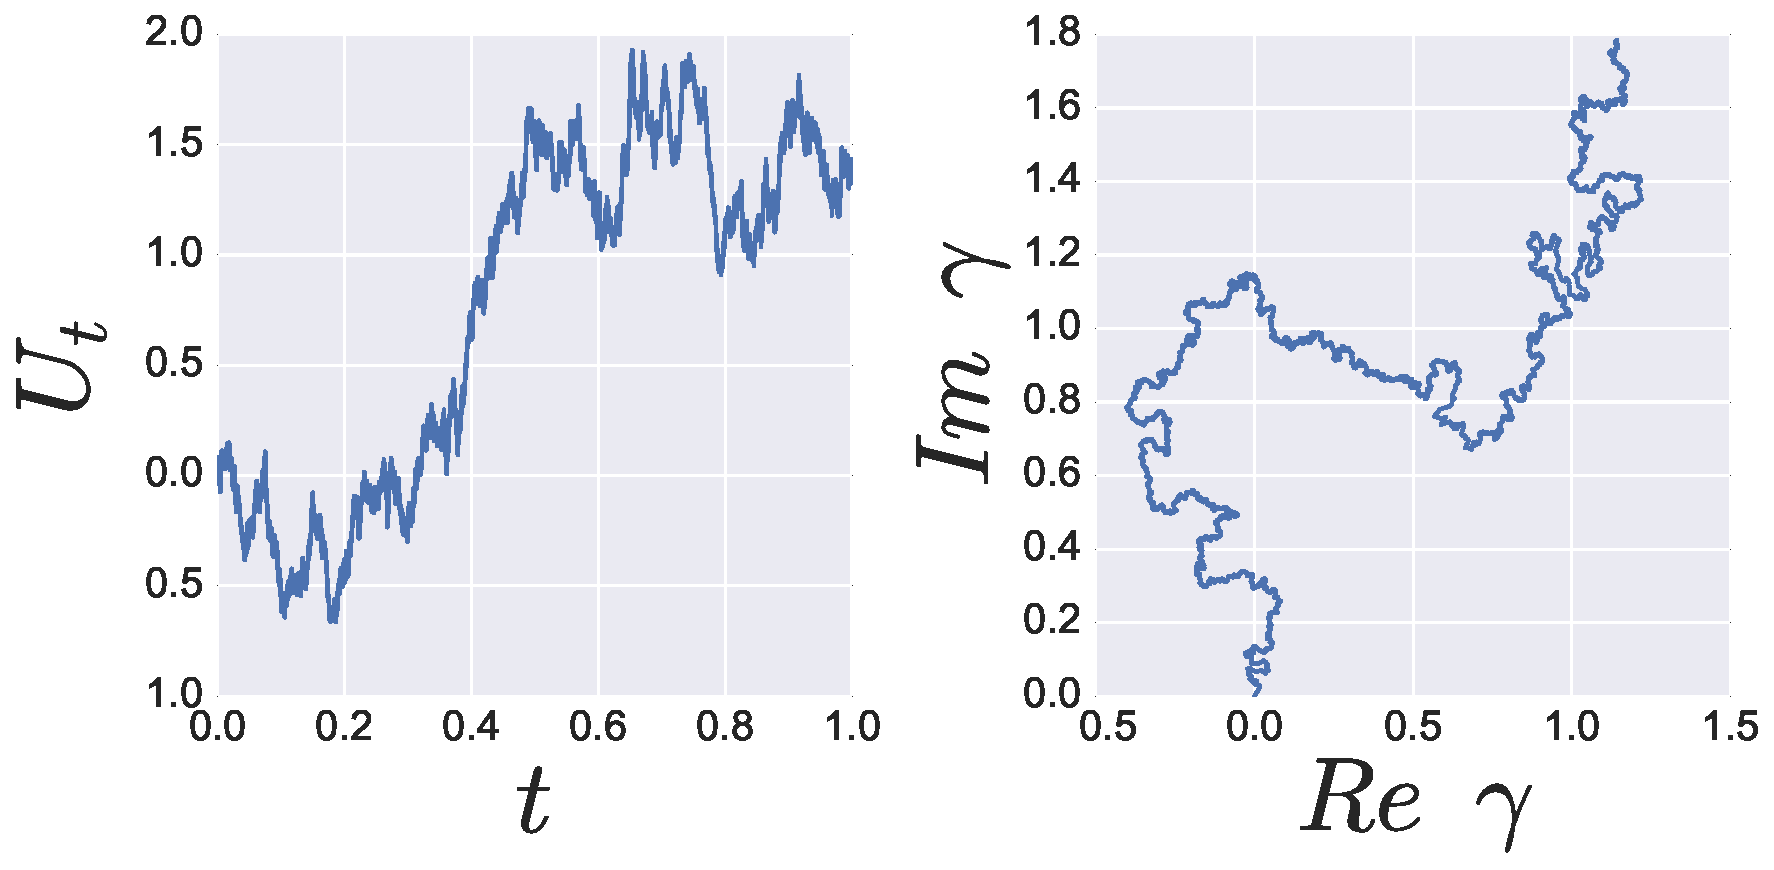
\includegraphics[width=\textwidth]{chapters/ch4-sle/figs/sleexample}
\end{center}
\caption{Example of a Schramm-Loewner evolution, which is a Loewner evolution
    driven by a Browninan motion, in this case with diffusion coefficient
    $\kappa=2$.}
\label{fig:sleexample}
\end{figure}

\begin{figure}
\begin{center}
    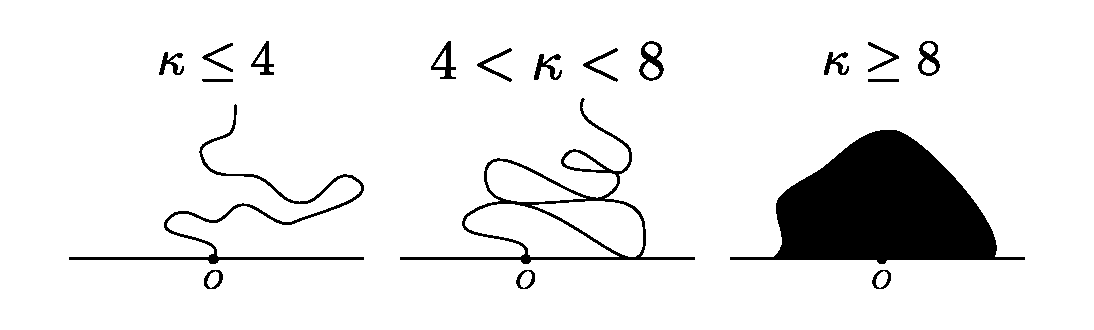
\includegraphics[width=\textwidth]{chapters/ch4-sle/figs/kappa}
\end{center}
\caption{The SLE trace display three different behaviors depending on the value
    of $\kappa$. For $\kappa\leq4$ the trace is simple, so it does not touch
    itself. For $4<\kappa<8$ the trace touches itself. And for $\kappa\geq8$
    the trace is space filling.}
\label{fig:kappa}
\end{figure}

\begin{figure}
\begin{center}
    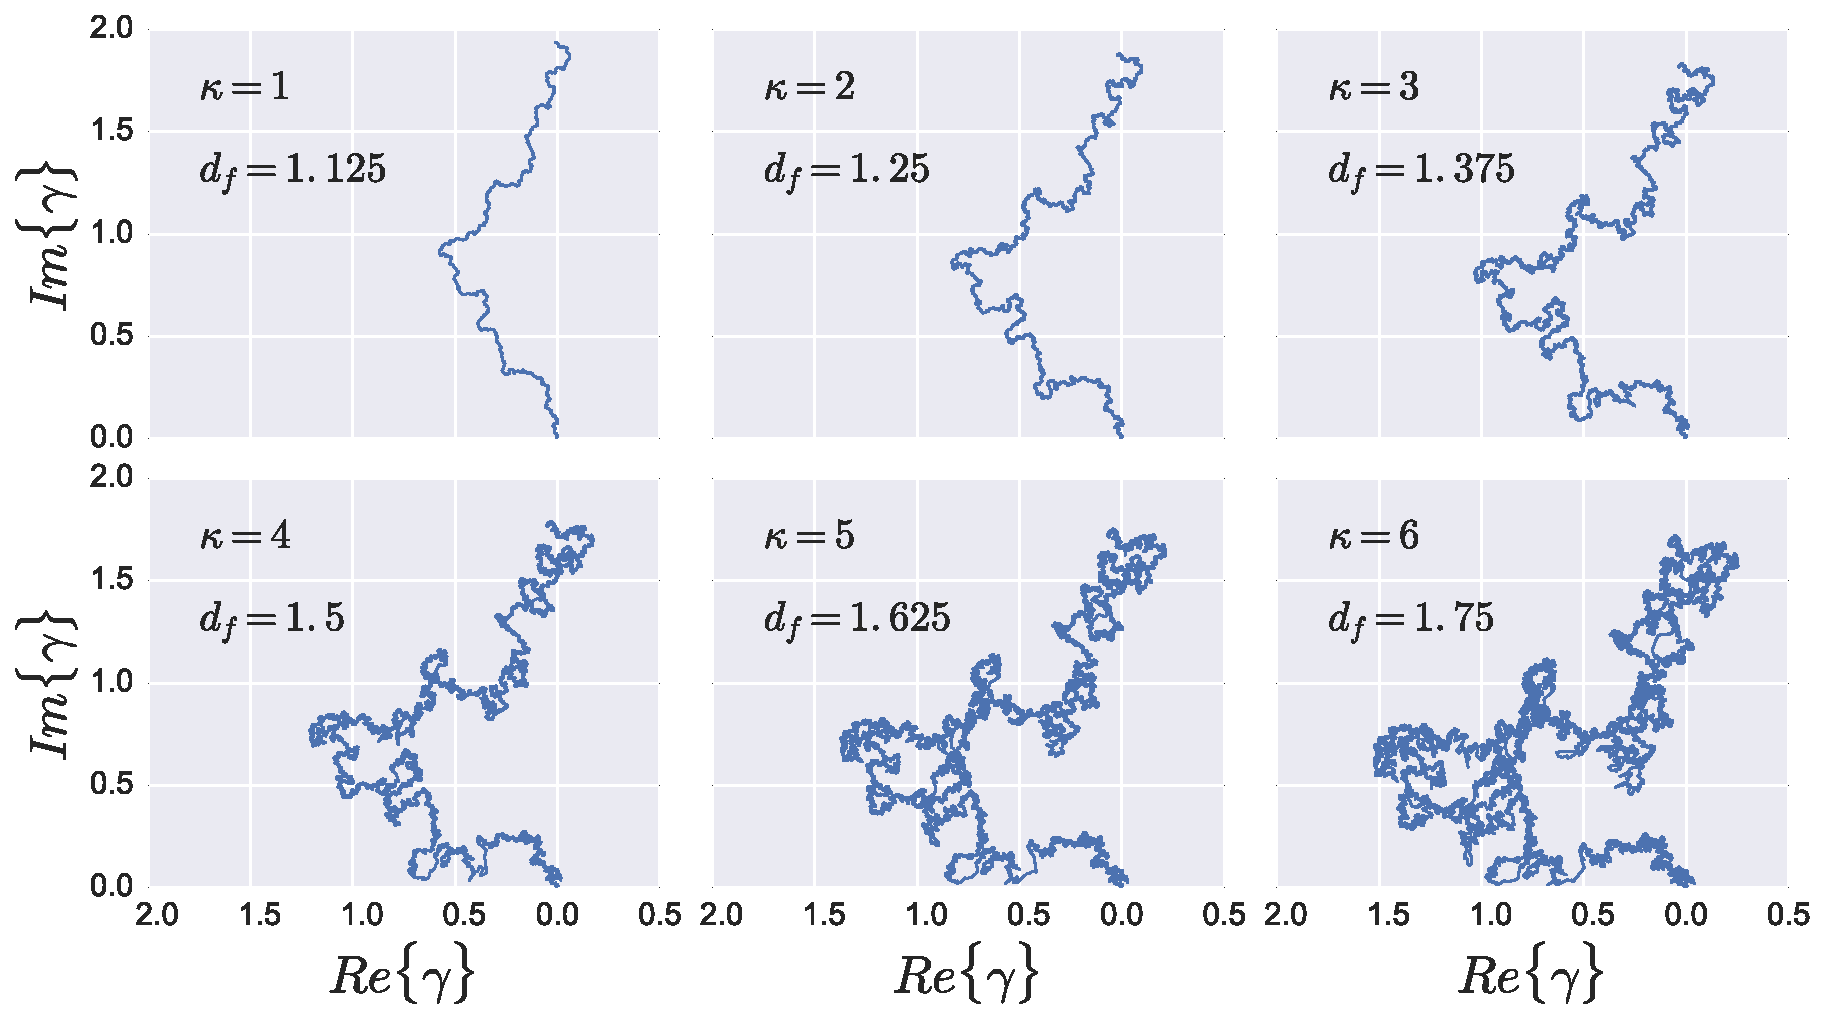
\includegraphics[width=\textwidth]{chapters/ch4-sle/figs/slefracdim}
\end{center}
\caption{Examples of several SLE traces generated using the same underlying
    Brownian motion, but with different $\kappa$. The fractal dimension is
    given by $d_f=\min(1+\kappa/8, 2)$.}
\label{fig:slefracdim}
\end{figure}


\section{Lévy Processes, Anomalous Diffusion, and SLE}
\label{sec:levy}

As mentioned so far, SLE is a theory concerned with conformally invariant
families of curves, which are always driven by a Brownian motion. In all other
cases, however, the curves themselves are not required to be conformally
invariant, even though the Loewner equation describes the time evolution of a
conformal map~\cite{Henkel2012}. This opens space for the study of stochastic
Loewner evolutions driven by processes that deviate from the Brownian motion.
This is the case of the work of Rushkin \textit{et al.}~\cite{Rushkin2006,
Oikonomou2008}, who studied SLE driven by L\'evy processes, $L_t$,
which behave pretty much like the Brownian motion described in
Section~\ref{sec:sle}, except the increments are distributed according to a
power law in the limit of large $x$
\begin{equation}
    P(L_{t+dt} - L_t \in [x, x+dx]) \propto \frac{1}{|x|^{1+\mu}}dxdt,
    \,\,\,\,\,\,\,\,\,\,
    0<\mu<2.
\end{equation}
In general, stochastic processes can be classified according 
to the behavior of the mean square displacement, which usually goes like
\begin{equation}
    \left\langle U_{t}^{2}\right\rangle \propto t^{\alpha}.
\end{equation}
For the Brownian motion, $\alpha=1$, which is referred as regular diffusion.
L\'evy processes are called superdiffusive because $\alpha=2/\mu>1$. Some
processes can also present the case $\alpha<1$, called subdiffusive. The exact
effect of the value of the diffusion exponent $\alpha$ on the properties of the
trace is yet unknown, but it was noted that the traces (which are not
continuous, for $L_t$ is also not continuous), present an anisotropic scaling
with time. This means the typical width and height of the hull, $X(t)$ and $Y(t)$
respectively, scale with different exponents following the relations
\begin{eqnarray}
    \label{eq:aniscale}
    X\left(t\right) & \sim & t^{1/\mu},\,\,\,0<\mu<2\\
    Y\left(t\right) & \sim & \begin{cases}
    A+Bt^{1-1/\mu}, & \mu\neq1\\
    \log\left(t\right), & \mu=1.
    \end{cases}
\end{eqnarray}


\section{Numerical Methods}
\label{sec:num}

The crux of the Schramm Loewner Evolution problem (at least from a physicist's
standpoint) is determining whether or not a given model converges to it in the
continuum limit, and what is the value of $\kappa$ for each specific model. We
mentioned several models that have show such convergence, the most illustrious
being Smirnov's demonstration that percolation in a triangular lattice is an
SLE with $\kappa=6$~\cite{Smirnov2001b}. Nonetheless, just like nobody would
expect every critical system to have an exact solution similar to the Ising
model, one may not expect to be able to prove the SLE convergence for every
conceivable model. This is where numerical analysis comes into the scene. By
comparing the statistical behavior of the model with the expected SLE trace, we
can infer if the hypothesis holds true.

In this section we will present some algorithms for computing Loewner
evolutions out of any given driving function, as well as the opposite task,
computing the driving function from any given trace.


\subsection{Euler's Method}
\label{ss:euler}

Euler's method for solving ordinary differential equations is arguably the
simplest~\cite{Press2007}. It is used to solve equation of the type $y'(t) =
f(y, t)$ and it basically consists in taking a first order approximation of the
solution
\begin{equation}
    \newcommand{\y}[1]{y\left(#1\right)}
    \newcommand{\f}[1]{f\left(#1\right)}
    \y{t} = \y{t_0} + \int_{t_0}^t \f{\y{\tau}, \tau} d\tau \approx
            \y{t_0} + \left(t - t_0\right)\f{\y{t_0}, t_0},
\end{equation}
as long as $t - t_0$ is small enough. This way, the equation can be solved
recursively by providing a discretized driving function $U_{t_i}$ with $t_0 =
0 < t_{1}<\cdots<t_N$ and. Applying it to Loewner's equation
(Eq.~\ref{eq:loew}) we have
\begin{equation}
    g_{t_{i+1}}(z) = g_{t_i}(z) + (t_{i+1} - t_i) \frac{2}{g_t(z) - U_{t_i}}.
\end{equation}

In order to obtain the trace from $g_t$ we take the fact that
\begin{equation}
    g_t(\gamma_t) = U_t.
    \label{eq:root}
\end{equation}
You can use your favorite method of root finding to solve Eq.~\ref{eq:root} for
$\gamma_t$. Figure~\ref{fig:euler1} shows a realization for $\kappa=2$. In it
we colored the grid according to the sign of $Re\{g_t(z)-U_t\}$. The border
between the positive and negative sides should be around the region where the
trace is. We also observe the most blatant drawback of the method: it fails in
several points, where they get mapped outside the upper half plane, which is
not allowed in chordal Loewner's evolutions. This problem accentuates quickly
as the value of $\kappa$ rises, to the point where the case $\kappa=6$
(Figure~\ref{fig:euler2}) has barely any discernible trace.

Other problem with Euler's method in the context of Loewner evolutions is
computational complexity. It requires $O(N)$ for each point of the space where
you compute $g_t(z)$, considering the you use a $(M,M)$ regular grid, the whole
algorithm have complexity $O(NM^2)$. This is further aggravated by the fact the
most points are not necessary to actually compute the trace, making most of the
computational effort useless. One possible advantage is the fact that this
algorithm is highly parallelizable, although this is hardly an advantage faced
with the other drawbacks.

\begin{figure}
\begin{center}
    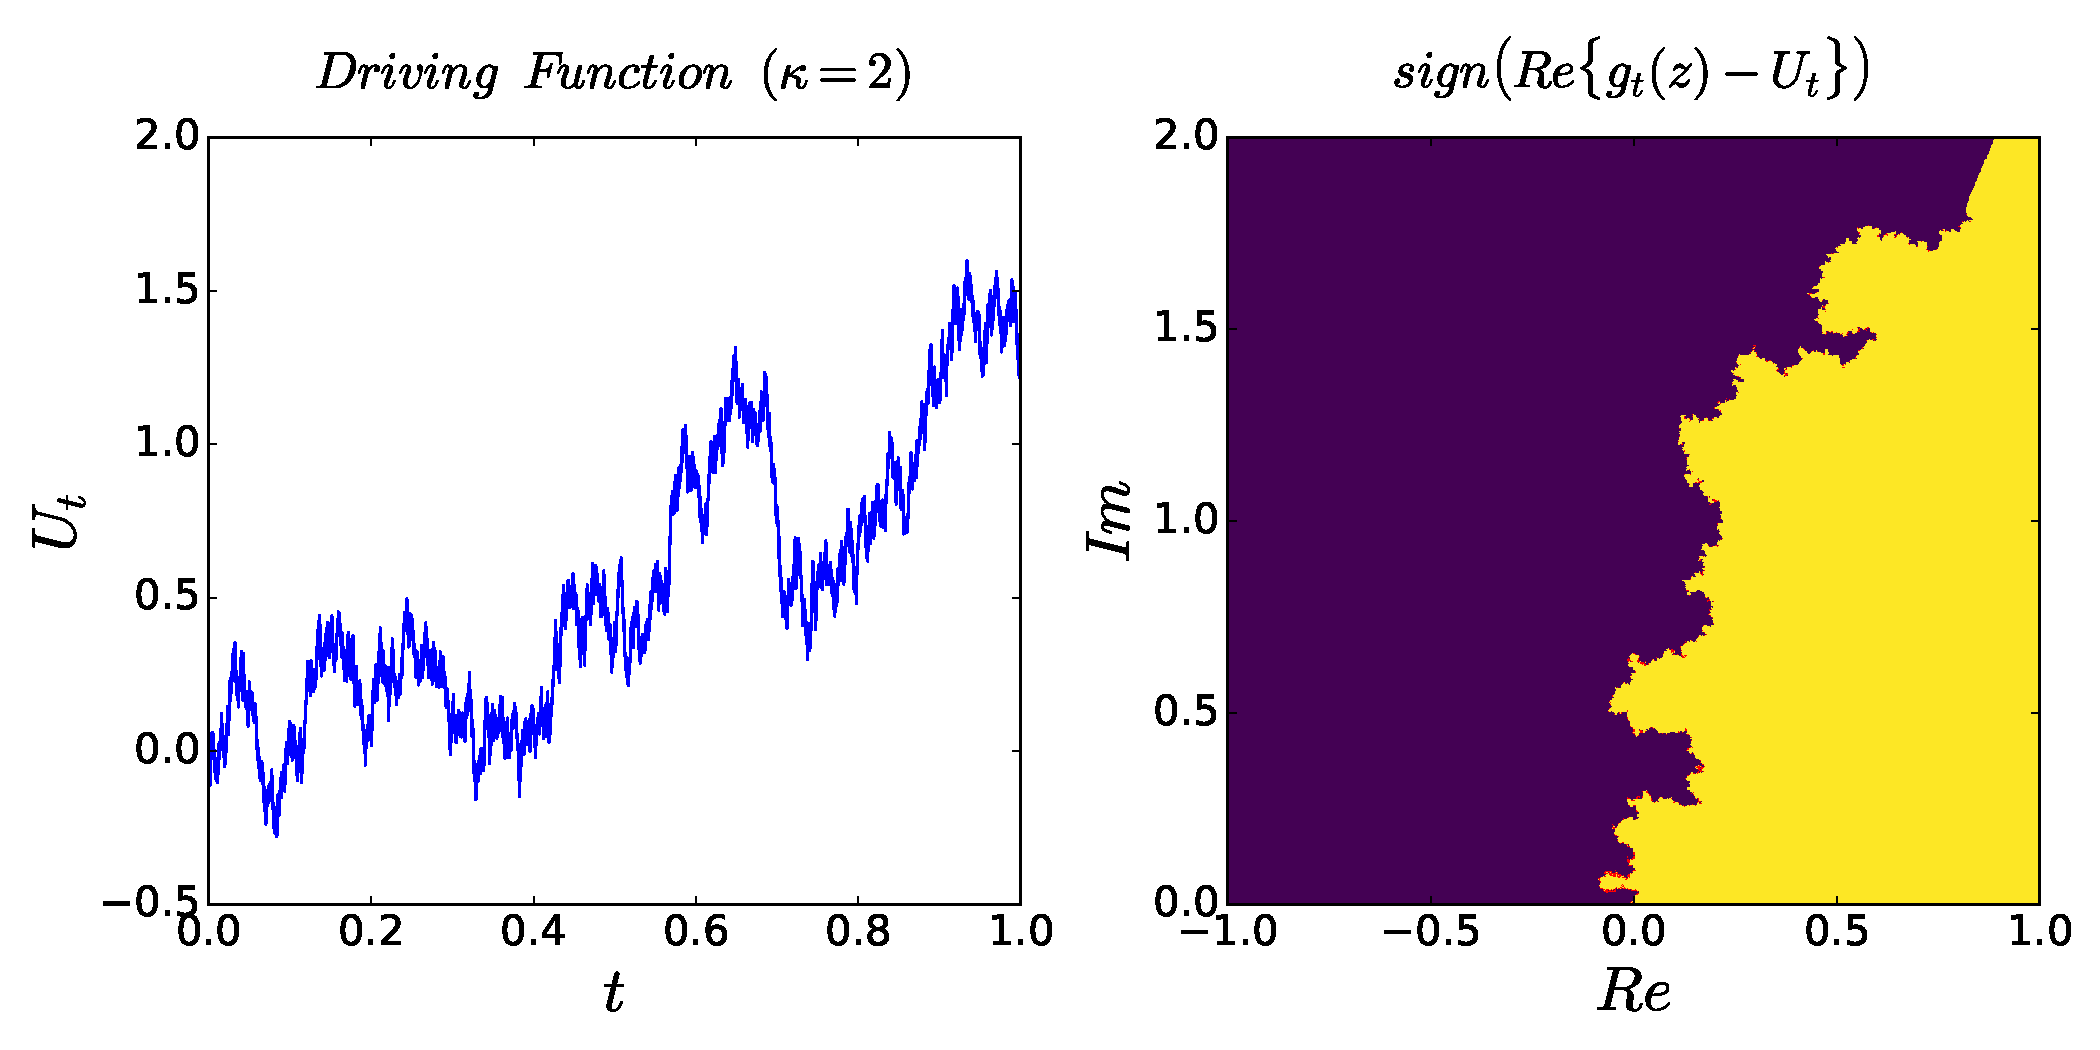
\includegraphics[scale=0.45]{chapters/ch4-sle/figs/euler1}
\end{center}
\caption{Simulation of an SLE process with $\kappa=2$ using the Euler method
    with $\Delta t = 10^{-5}$ in a grid of resolution $(1024, 1024)$. Because
    at time $t$ $g_t(\gamma_t)-U_t=0$, if we color the upper half plane
    according to which side of the real line each point is mapped, the border
    between the regions should indicate the position of the trace $\gamma_t$.
    The red points are the points where the method failed and were mapped
    outside the upper half plane. The smooth ``tail'' of the trace happens
    because these points have not yet been mapped to the real line.}
\label{fig:euler1}
\end{figure}

\begin{figure}
\begin{center}
    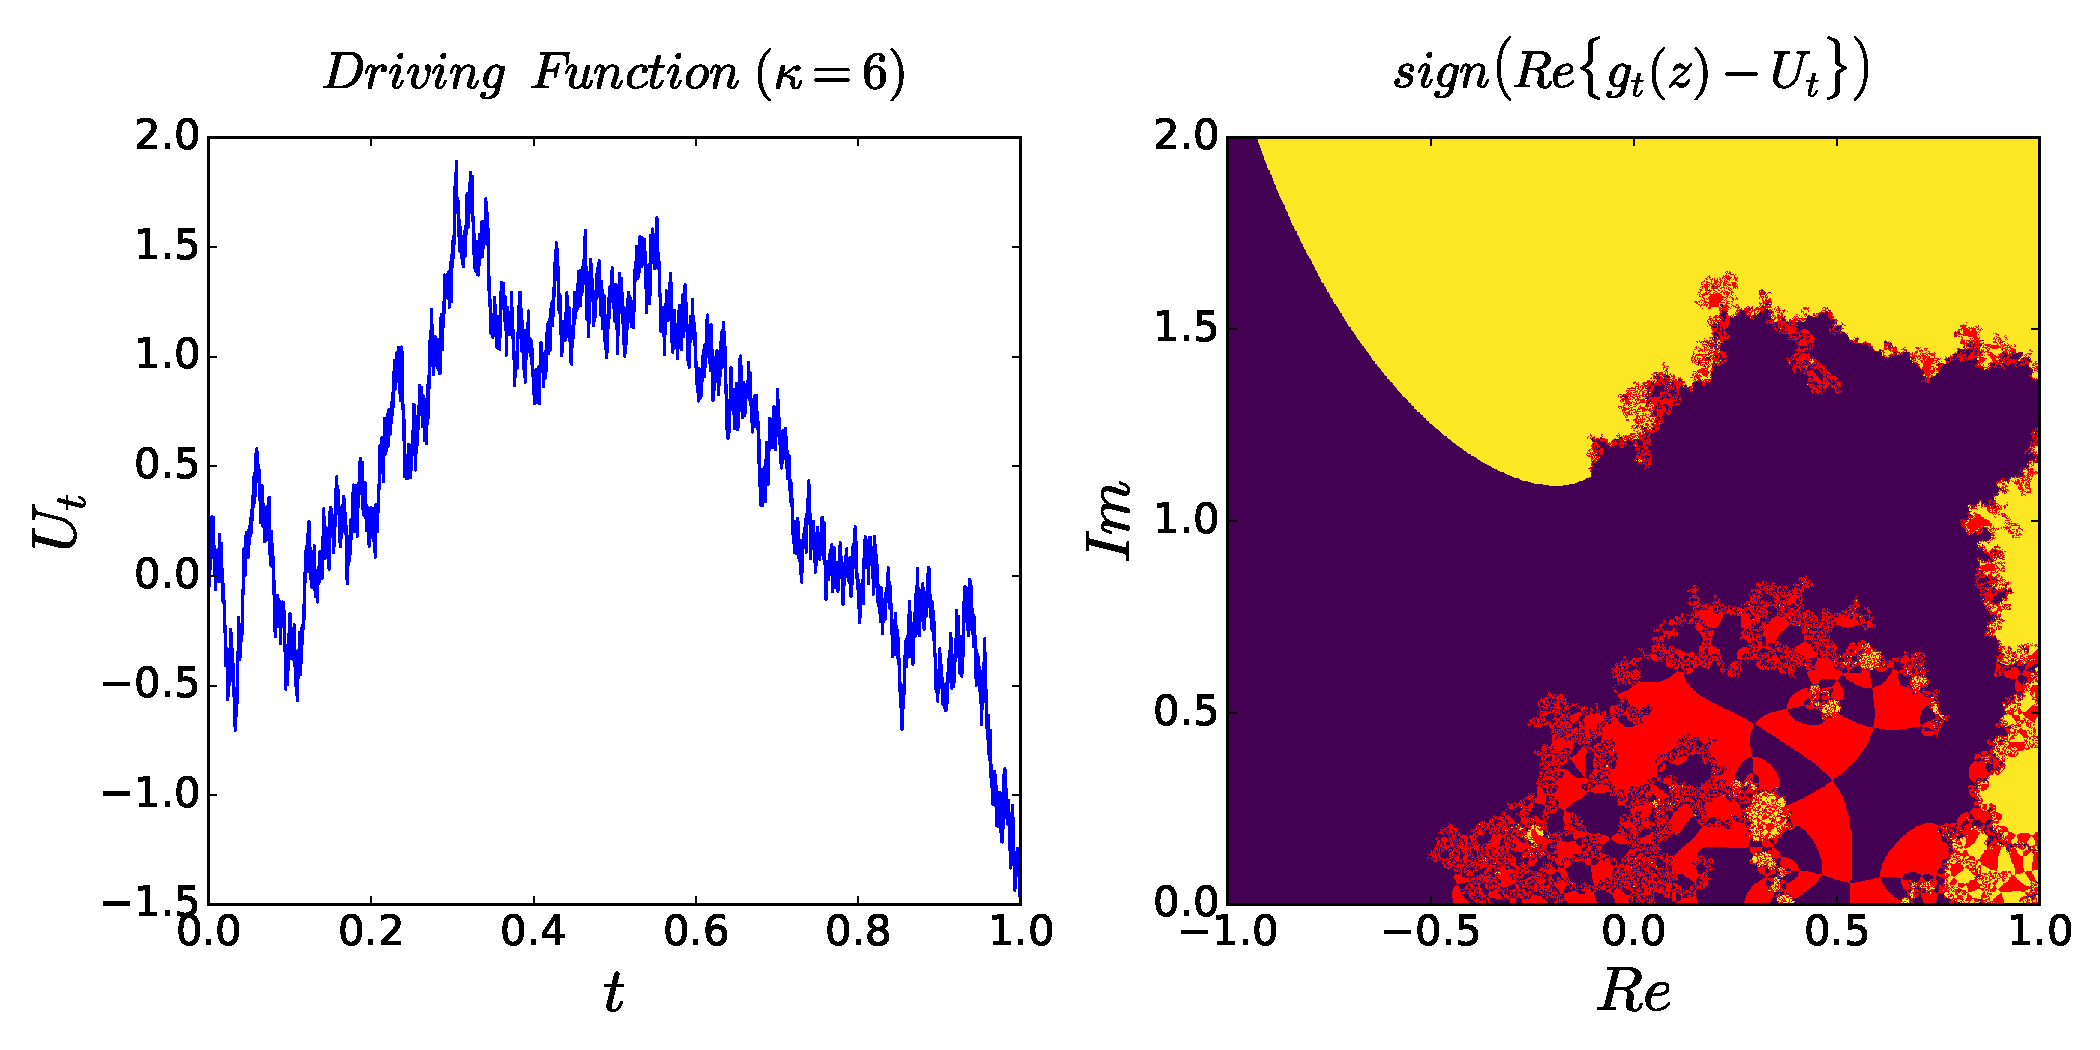
\includegraphics[scale=0.45]{chapters/ch4-sle/figs/euler2}
\end{center}
\caption{Simulation of an SLE process with $\kappa=6$ using the Euler method
    with $\Delta t = 10^{-5}$ in a grid of resolution $(1024, 1024)$. 
    The red points are the points where the method failed and were mapped
    outside the upper half plane. The algorithm performed much worse than
    the case $\kappa=2$.}
\label{fig:euler2}
\end{figure}


\subsection{Zipper Algorithm}
\label{ss:zipper}

Since the Euler's method perform so poorly in the task of computing the SLE
trace, a better method is needed. The one described here is called the
\textit{zipper algorithm}, and it's used throughout this work. It is based on
the idea of discrete Loewner evolutions~\cite{Bauer2003, Kennedy2009}, series
of smaller simpler Loewner evolutions.

For starters, we take a driving function $U_t$ sampled in a set of $N+1$ time
instants $0=t_0<t_1<\cdots<t_N$. As we already established, the solution of the
Loewner's equation for $U_t$ is $g_t$, which maps
$\HH\setminus\gamma_{\left[0,t_{k}\right]}$ to $\HH$. We then define the
helper function
\begin{equation}
    G_{k}=g_{t_{k}}\circ g_{t_{k-1}}^{-1},
\end{equation}
which maps $\HH\setminus\gamma_{\left[0,t_{k-1}\right]}$ to
$\HH\setminus\gamma_{\left[0,t_{k}\right]}$. This way the solution of Loewner's
equation can be rewritten
\begin{equation}
    g_{t_{k}}=G_{k}\circ G_{k-1}\circ\cdots\circ G_{2}\circ G_{1}.
\end{equation}
The $G_k$ however are not solutions of Loewner's equation, as the trace they
generate do not start at the origin. We fix that by shifting the function by
$U_{t_{k-1}}$
\begin{equation}
    g_{k}=G_{k}\left(z+U_{t_{k-1}}\right)-U_{t_{k-1}}.
\end{equation}
Note that in the notation adopted (taken from~\cite{Kennedy2009}) $g_{t_k}$ and
$g_k$ are different functions. The $g_k$ are the solution of Loewner's equation
with driving function $\tilde{U}_t$ such that $\tilde{U}_0=0$ and
$\tilde{U}_{\Delta t_k} = \Delta U_k$, where $\Delta t_k = t_{k} - t_{k-1}$ and
$\Delta U_{k} = U_{k} - U_{k-1}$. Since we are trying to construct the trace
starting from the drive, we need to take the inverse of $g_k$
\begin{equation}
    f_{k}=G_{k}^{-1}\left(z+U_{t_{k-1}}\right)-U_{t_{k-1}}.
\end{equation}
The $k$-th point of the trace $\gamma_{t_k}$ is then determined by 
\begin{equation}
    \gamma_{t_k} = f_1(\cdots f_{k-1}(f_k(\Delta U_k)+\Delta U_{k-1})\cdots+\Delta U_1).
\end{equation}
For convenience we define
\begin{equation}
    h_{k}=f_{k}\left(z+\Delta U_{k}\right),
\end{equation}
so the $\gamma_t$ can be computed by applying the relation
\begin{equation}
    \label{eq:zip}
    \gamma_{k}=h_{1}\circ h_{2}\circ\cdots\circ h_{k}\left(0\right).
\end{equation}
If this helper function zoo looks confusing, Figure~\ref{fig:zipperdiag} shows
where they fit in the actual Loewner evolution process taking place.

Once the functional form of the $h_k$ is know, the algorithm is surprisingly
simple, it just consists of applying Eq.~\ref{eq:zip} for each value of $k$.
The form of $h_k$ however is dependent on the interpolation drive $\tilde{U}$.
The choice is basically free, however a convenient one should have an
analytical solution. The two most common are the vertical and tilted slits.

The vertical slit is done by making
\begin{equation}
    \tilde{U}(t)=\Delta U,
\end{equation}
which generate a vertical trace going from $\Delta U$ to $\Delta U +
i2\sqrt{\Delta t}$. This isn't strictly a Loewner evolution because the trace
does not start at the origin, but this is a numerical approximation where the
actual trace is a composition of many vertical slits, and the limit $\Delta t
\rightarrow 0$ converges to an actual SLE trace. The $h_k$ in this case is
given by~\cite{Kager2004b}
\begin{equation}
    \label{eq:vslit}
    h_{k}(z)=i\sqrt{4\Delta t-z^{2}}+\Delta U.
\end{equation}

The tilted slit is done by interpolating the drive with the function.
\begin{equation}
    \tilde{U}(t)=
        \frac{2\left(1-2\alpha\right)}
             {\sqrt{\alpha\left(1-\alpha\right)}}
        \sqrt{t}
\end{equation}
where
\begin{equation}
    \alpha=\frac{1}{2}-
    \mbox{sign}\left(\Delta U\right)\frac{1}{2}\sqrt{\frac{v}{16+v}},
    \,\,\,\,\,\,\,\,\,\,\,\,\,\,
    v=\frac{\Delta U^{2}}{\Delta t}.
\end{equation}
It generates a trace that is a tilted line that starts at the origin makes an
angle $\alpha\pi$ with the positive real line. The $h_k$ in this case is
given by
\begin{equation}
    h_{k}(z) = 
    {\left(
        z+2\sqrt{\frac{\left(1-\alpha\right)\Delta t}{\alpha}}
    \right)}^{1-\alpha}
    {\left(
        z-2\sqrt{\frac{\alpha\Delta t}{1-\alpha}}
    \right)}^{\alpha}.
\end{equation}
This discretization is more rigorous than the vertical slit, however in
practice they yield very similar results. See Figure~\ref{fig:zipper} for an
illustration of the whole process of applying repeated tilted slits to obtain
an SLE trace.

You can see in Figure~\ref{fig:eulerzip} how the zipper algorithm performs in
the high $\kappa$ regime. The result is not perfect, the jump size
$\left|\gamma_{k}-\gamma_{k-1}\right|$ is very non-uniform due to the high
volatility of the driving function. Nevertheless, the result is still much
better than the one obtained by using Euler's method, and the defects can be
mitigated by simply adding more points to the discretized driving function.
This is not so simple, however. Since each $k$-th point require $k$ application
of the $h_i$, the algorithm scales as $O(N^2)$, which can get unwieldy for very
large $N$. One possible solution is making use of parallelization, since each
$\gamma_k$ can be computed independently from one another. There's also more
complex approximative algorithms with better time complexity, up to
$O(N^{1.4})$~\cite{Kennedy2007}.

The next challenge is to do the opposite task, obtaining a driving function
from a given trace $\gamma_k$. This is much simpler when using a vertical slit.
First let's invert Equation~\ref{eq:zip}
\begin{equation}
    \label{eq:unzip1}
    0=h_{k}^{-1}\circ h_{k-1}^{-1}\circ\cdots h_{1}^{-1}\left(\gamma_{k}\right).
\end{equation}
We know that the vertical slit maps the origin to $\Delta U+i2\sqrt{\Delta t}$,
that is
\begin{equation}
    \label{eq:unzip2}
    h_{k}\left(0\right)=\Delta U+i2\sqrt{\Delta t}.
\end{equation}
Combining Eq.~\ref{eq:unzip1} and Eq.~\ref{eq:unzip2} we have    
\begin{equation}
    \Delta U_{k}+i2\sqrt{\Delta t_{k}}=
    h_{k-1}^{-1}\circ\cdots h_{1}^{-1}\left(\gamma_{k}\right).
\end{equation}
This way we can determine the $t_k$ and $U_{t_k}$ of given discretized
trace by simply taking
\begin{equation}
    \label{eq:unzip1}
    U_{t_k}=\sum_{i=1}^{k}\mbox{Re}\left\{ \omega_{i}\right\},
    \,\,\,\,\,\,\,\,\,\,
    t_{k}=\frac{1}{4}\sum_{i=1}^{k}\mbox{Im}\left\{ \omega_{i}\right\} ^{2}
\end{equation}
where
\begin{equation}
    \omega_{k}=h_{k-1}^{-1}\circ h_{k-2}^{-1}\circ
        \ldots\circ h_{1}^{-1}\left(\gamma_{k}\right).
\end{equation}
The $h_k^{-1}$ can be easily determined by inverting Eq.~\ref{eq:vslit}
\begin{equation}
    h_{k}^{-1}\left(z\right)=
    i\sqrt{-Im{\left\{ \omega_{k}\right\}}^{2}
           -{\left(z-\mbox{Re}\left\{ \omega_{k}\right\} \right)}^{2}}.
\end{equation}

\begin{figure}
\begin{center}
    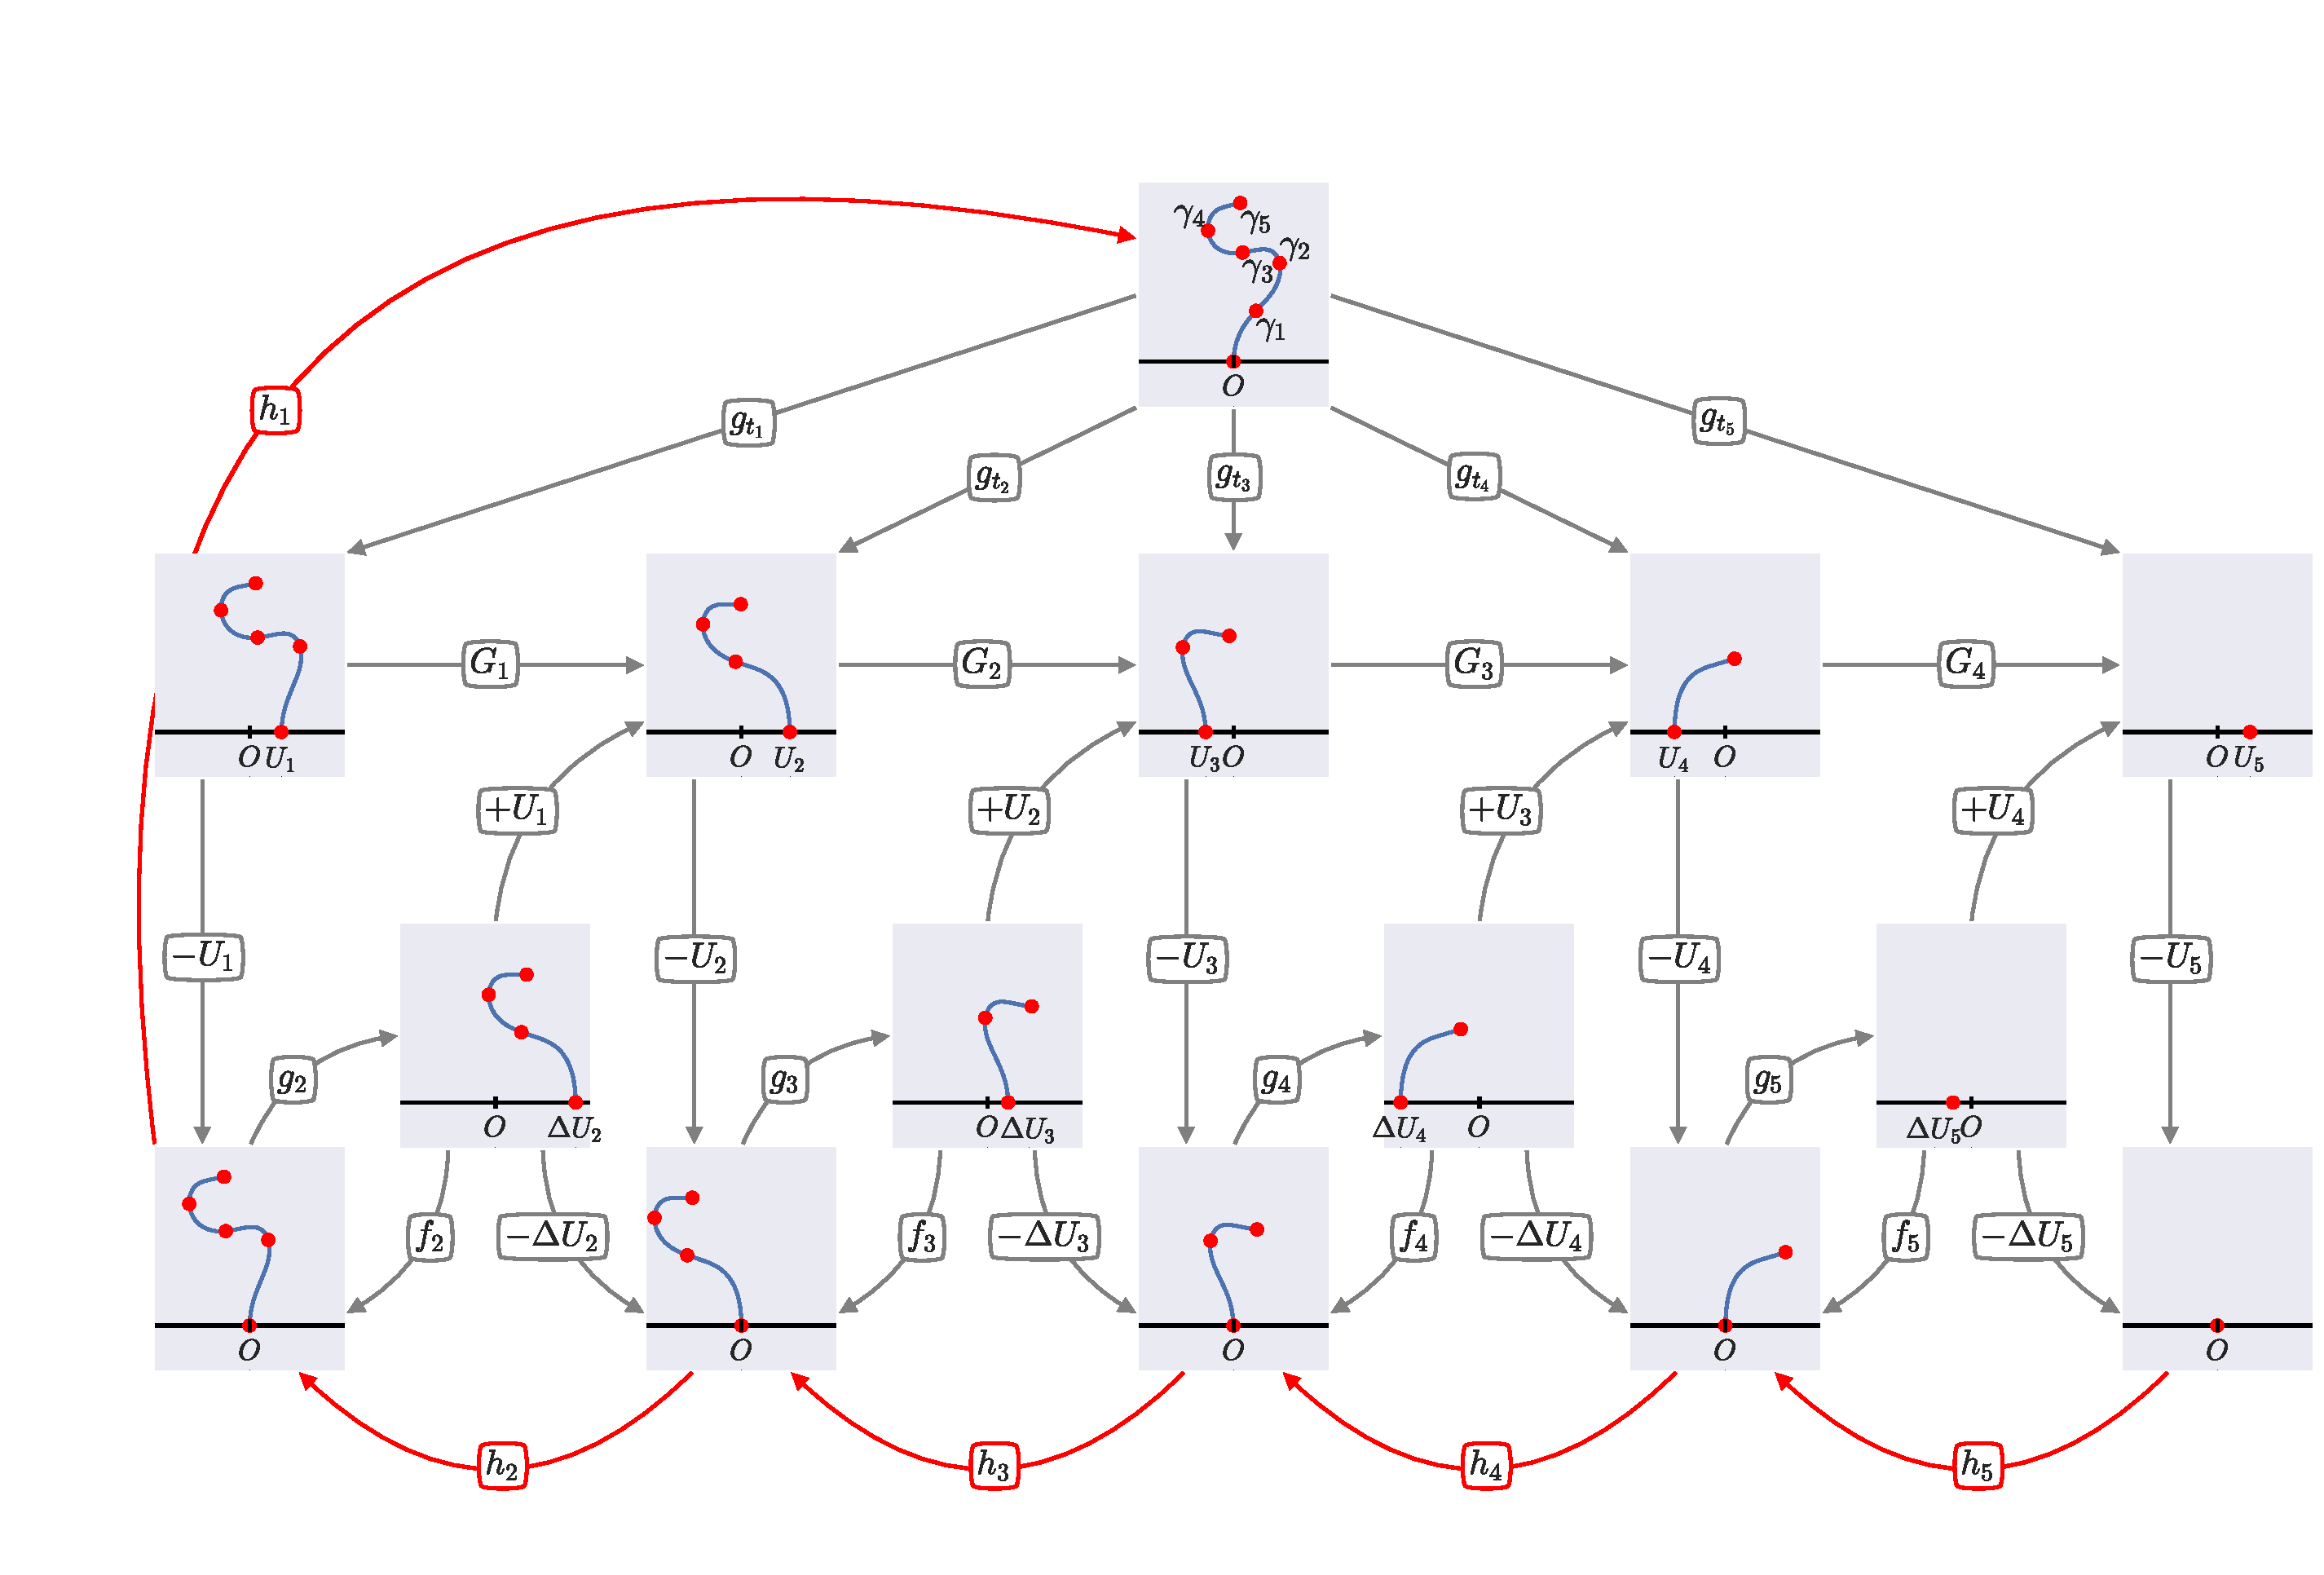
\includegraphics[width=\textwidth]{chapters/ch4-sle/figs/zipperdiag}
\end{center}
\caption{Schematic representation of how the zipper algorithm fits in the
    Loewner evolution framework. At the top, we have the full trace up to time
    $t_5$, which we want to reach starting from the empty upper half plane
    (right most panel on the fourth row). To compute the trace from a given
    discretized driving function, one must take the red path. This is achieved
    by using the interpolating maps $g_i$ that are the solution of the Loewner
    equation with driving function $\tilde{U}_0=0$ and $\tilde{U}_{\Delta
    t}=\Delta U$. The choice of interpolation function $\tilde{U}$ is
    arbitrary, but usually taken from the few options that have an analytical
    solution.}
\label{fig:zipperdiag}
\end{figure}

\begin{figure}
\begin{center}
    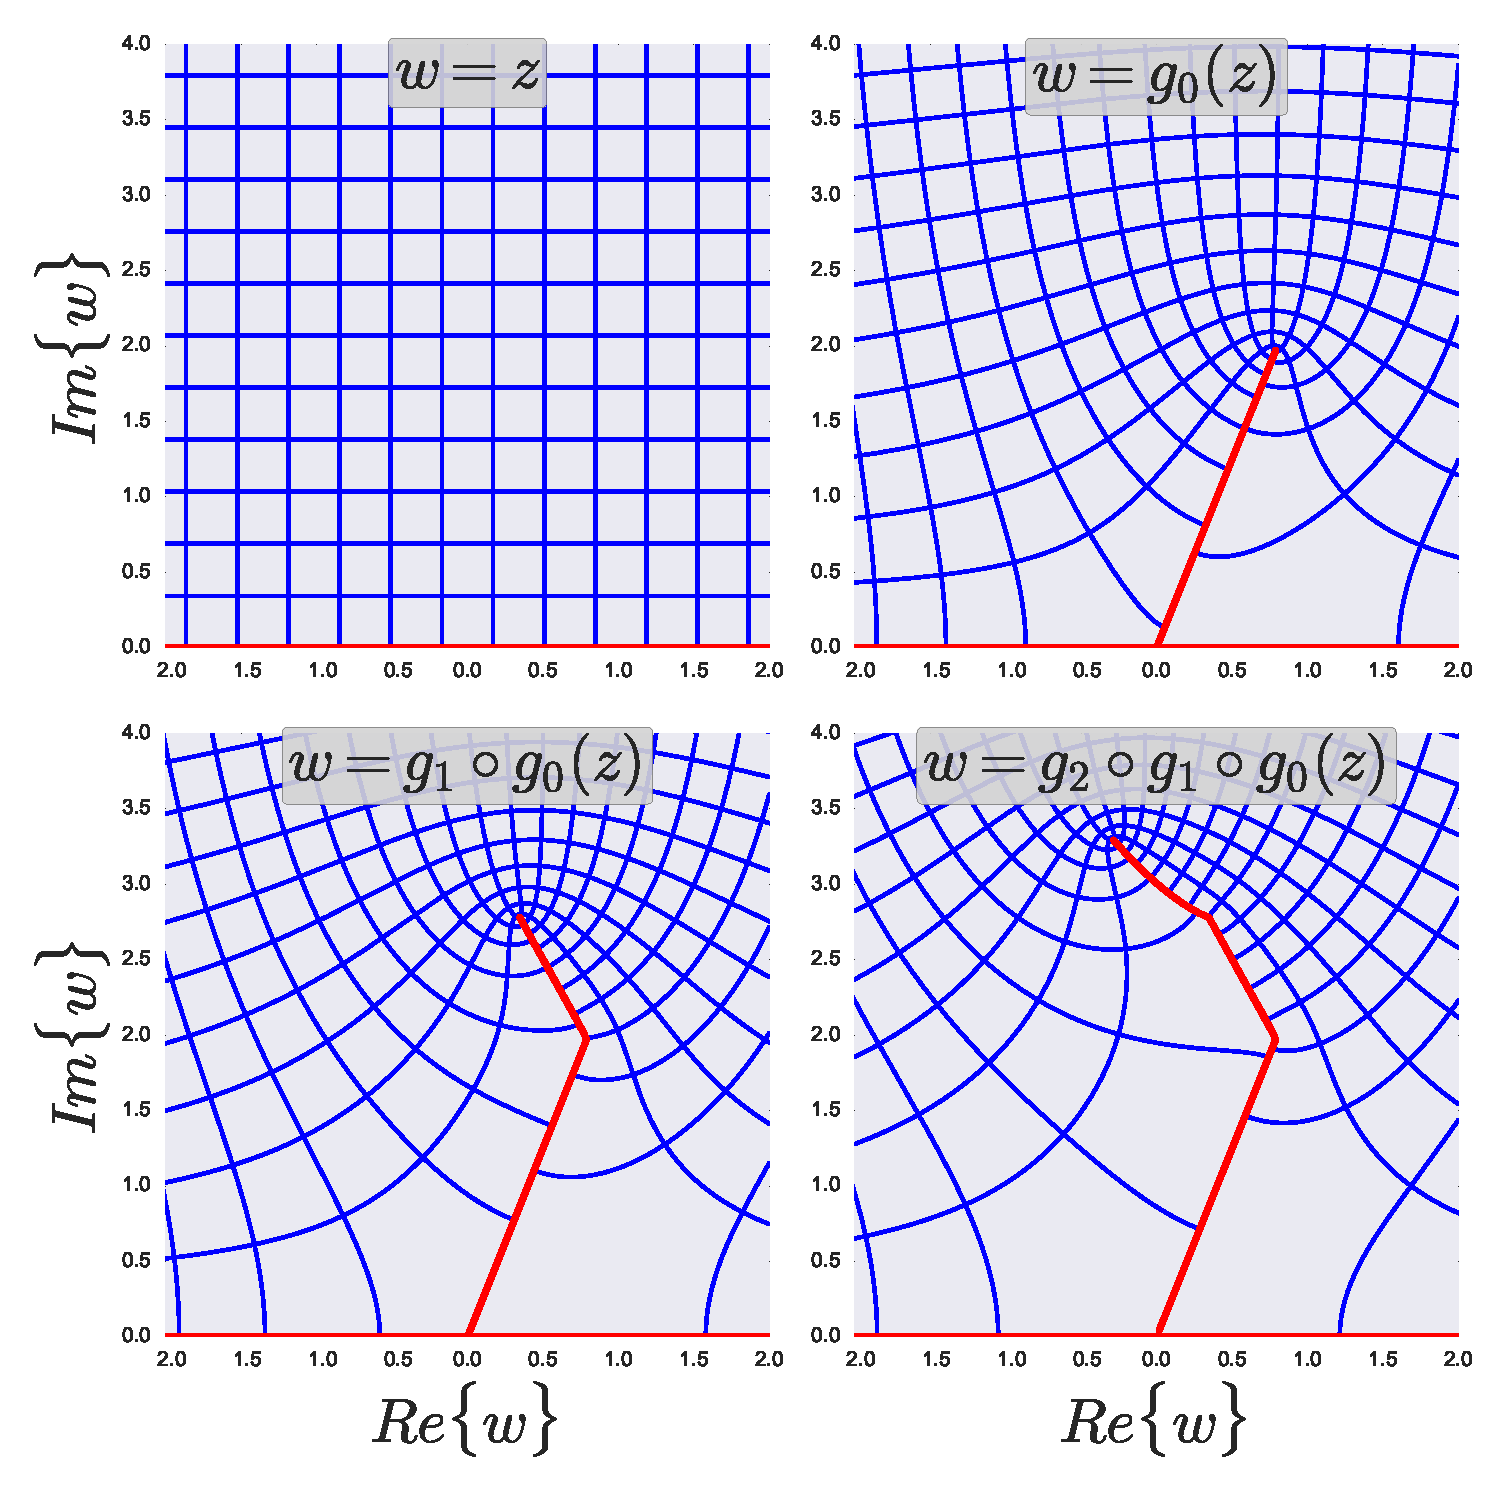
\includegraphics[scale=0.5]{chapters/ch4-sle/figs/zipper}
\end{center}
\caption{Result of applying the first three iterations of the zipper algorithm
    with the tilted slit approximation. In the limit $\Delta t\rightarrow 0$
    the red line converges to an SLE trace.}
\label{fig:zipper}
\end{figure}

\begin{figure}
\begin{center}
    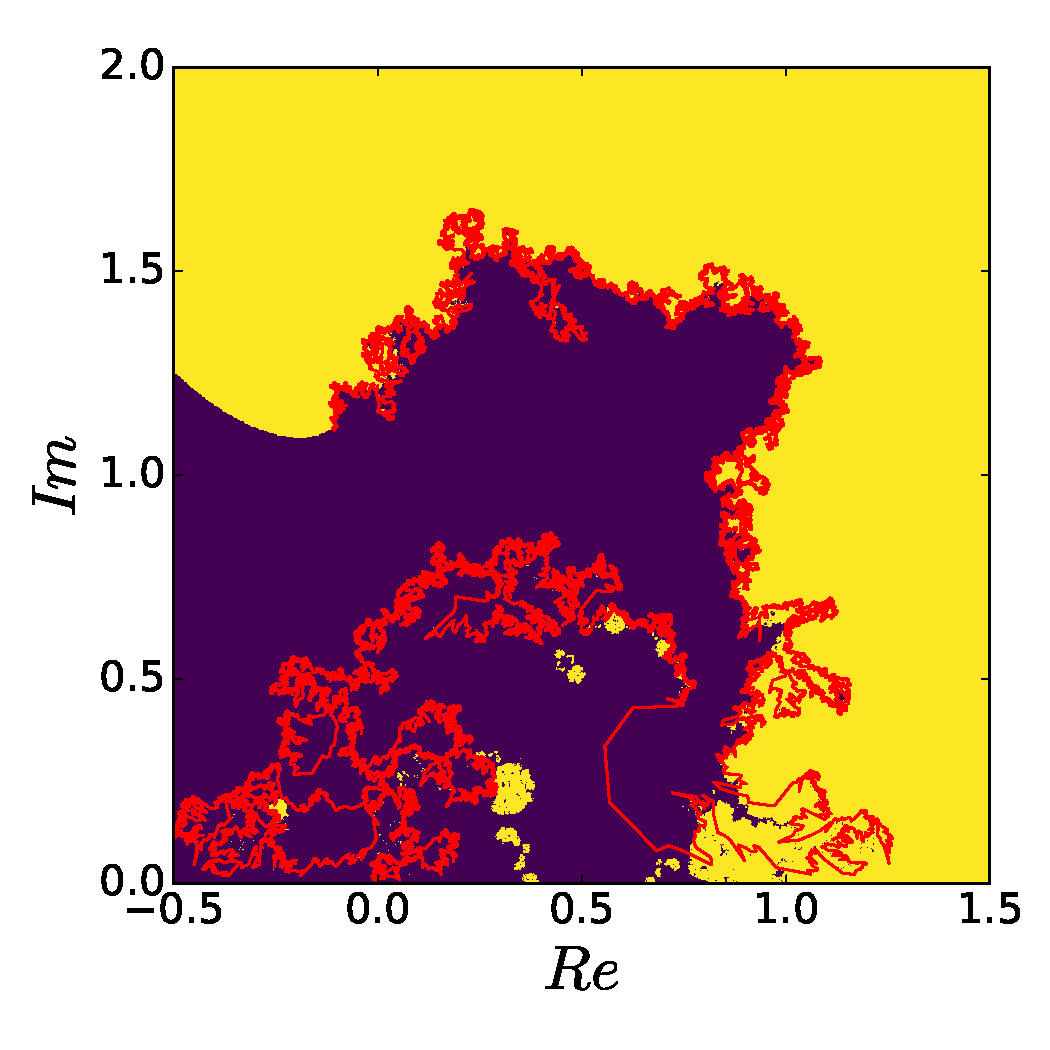
\includegraphics[scale=0.5]{chapters/ch4-sle/figs/eulerzip}
\end{center}
\caption{Comparison of the traces obtained by using the zipper algorithm (red
    line) and Euler's method. Although it presents large jumps in the trace due
    to large displacements in the driving function, zipper it still performs
    better than the Euler's.}
\label{fig:eulerzip}
\end{figure}
